\chapter{Stochastic switching linear control using nonlinear hybrid models}
\label{sec_spf_control}
We continue our discussion of switching controller algorithms from chapter \ref{sec_rbpf_control} here. In this chapter we use the switching particle filter to identify the best model to use in the stochastic controllers we developed in chapter \ref{sec_linear_control}. More precisely, let $M_i = (A_i, B_i)$ be the linearised model corresponding to the nonlinear models $(f_i, g_i)$ as discussed in chapter \ref{sec_inf_spf}. By finding the most likely nonlinear model, using the switching particle filter, we aim to design a linear controller (based on the most likely nonlinear model) which is robust against system faults.

The fundamental difference between the controllers we develop in this chapter and those of chapter \ref{sec_rbpf_control} is that the linear model used for state prediction is, if the filter behaves as intended, an accurate approximation of the underlying dynamics. In chapter \ref{sec_rbpf_control} the controllers performed poorly because they were used to predict the system states into regions where they were not accurate. In this chapter we use the switching particle filter to identify when the underlying dynamics change. The more accurate model is then used for control; however, the crucial difference is that we do not attempt to traverse the state space as in chapter \ref{sec_rbpf_control}. We rather solve the more modest goal of keeping the system at set point in the presence of system faults. 

We assume the same scenario as introduced in section \ref{sec_spf_filtering} i.e. we assume we have 2 nonlinear plant models available. Model $M_1$ corresponds to the healthy CSTR and model $M_2$ corresponds to the CSTR with denatured catalyst (the faulty model). We will again avail ourselves of the switching controller algorithm  repeated here for convenience.

\textbf{Switching controller algorithm}:
\begin{enumerate}
\item
Use a switching filter algorithm, e.g. the switching particle filter, to update the state estimates of the particle population given the current observation. See chapter \ref{sec_inf_spf} for more details.
\item
Select the particle with the highest switching weight. Since each particle corresponds to a certain model we implicitly have the most probable model $M_i$.
\item
Use the mean and covariance information encoded by this particle within the context of the stochastic controller (LQG or MPC) formulation of chapter \ref{sec_linear_control}. Use the most likely model, $M_i$ from step 2, in this setting.
\item
Repeat for the next observation. 
\end{enumerate} 
A coincidental benefit of this approach is that the filter/controller combination will automatically detect the modelled fault. We do not consider the model averaging approach (in finding the best linear model to use for control) because it will not make physical sense: the plant is either healthy or broken but cannot be a mixture between the two.

Since the underlying graphical model in chapter \ref{sec_inf_lin_hybrid} and chapter \ref{sec_inf_spf} is the same, we expect the filtering trends to be the same as those found in chapter \ref{sec_inf_lin_hybrid}. For the sake of illustration we exclusively use both state measurements. There is no fundamental reason why one cannot use only one state measurement except that the filter performance will be worse.

For the remainder of this chapter we assume the control goal is to keep the system at the unsteady concentration operating point of the healthy model, even in the presence of the denatured catalyst. In all the simulations the catalyst denatures at 100 minutes. This allows us to demonstrate that the switching controller is able to regulate both the healthy and faulty plant. 

\section{Unconstrained switching control}
\label{sec_spf_uncon}
In this chapter we compare the LQG controller (discussed in sections \ref{sec_lqg_lit} and \ref{sec_uncon_lin_control}) to the switching controller algorithm implemented within the context of the LQG controller
\begin{equation}
\begin{aligned}
&\underset{\mathbf{u}}{\text{min }} \mathbb{E}\left[ \frac{1}{2}\sum_{k=0}^{N-1} \left( x_k^TQx_k + u_k^TRu_k \right) + \frac{1}{2}x_N^TP_fx_N \right] \\
& \text{subject to } x_{t+1}=A_ix_t+B_iu_t + w_t.
\end{aligned}
\label{eq_spf_lqg}
\end{equation}
For the non-switching LQG controller we use a particle filter to estimate the current state. The same control parameters as those found in section \ref{sec_lin_sys_cont} are used. Note that the current state estimate $x_0$ is inferred from the respective observers. Note that we select the most likely model, $M_i=(A_i, B_i)$, based on the switch weight supplied by the switching particle filter at each time step. This model is then used in (\ref{eq_spf_lqg}) and solved using the techniques of section~\ref{sec_uncon_lin_control}.
 
In figure \ref{fig_spf_pf_lqg_track} we see the performance of the LQG controller applied to the CSTR system. At 100 minutes the catalyst denatures and the model used to design the controller becomes grossly inaccurate. The inappropriateness of the model also affects the particle filter's performance. 
\begin{figure}[H] 
\centering
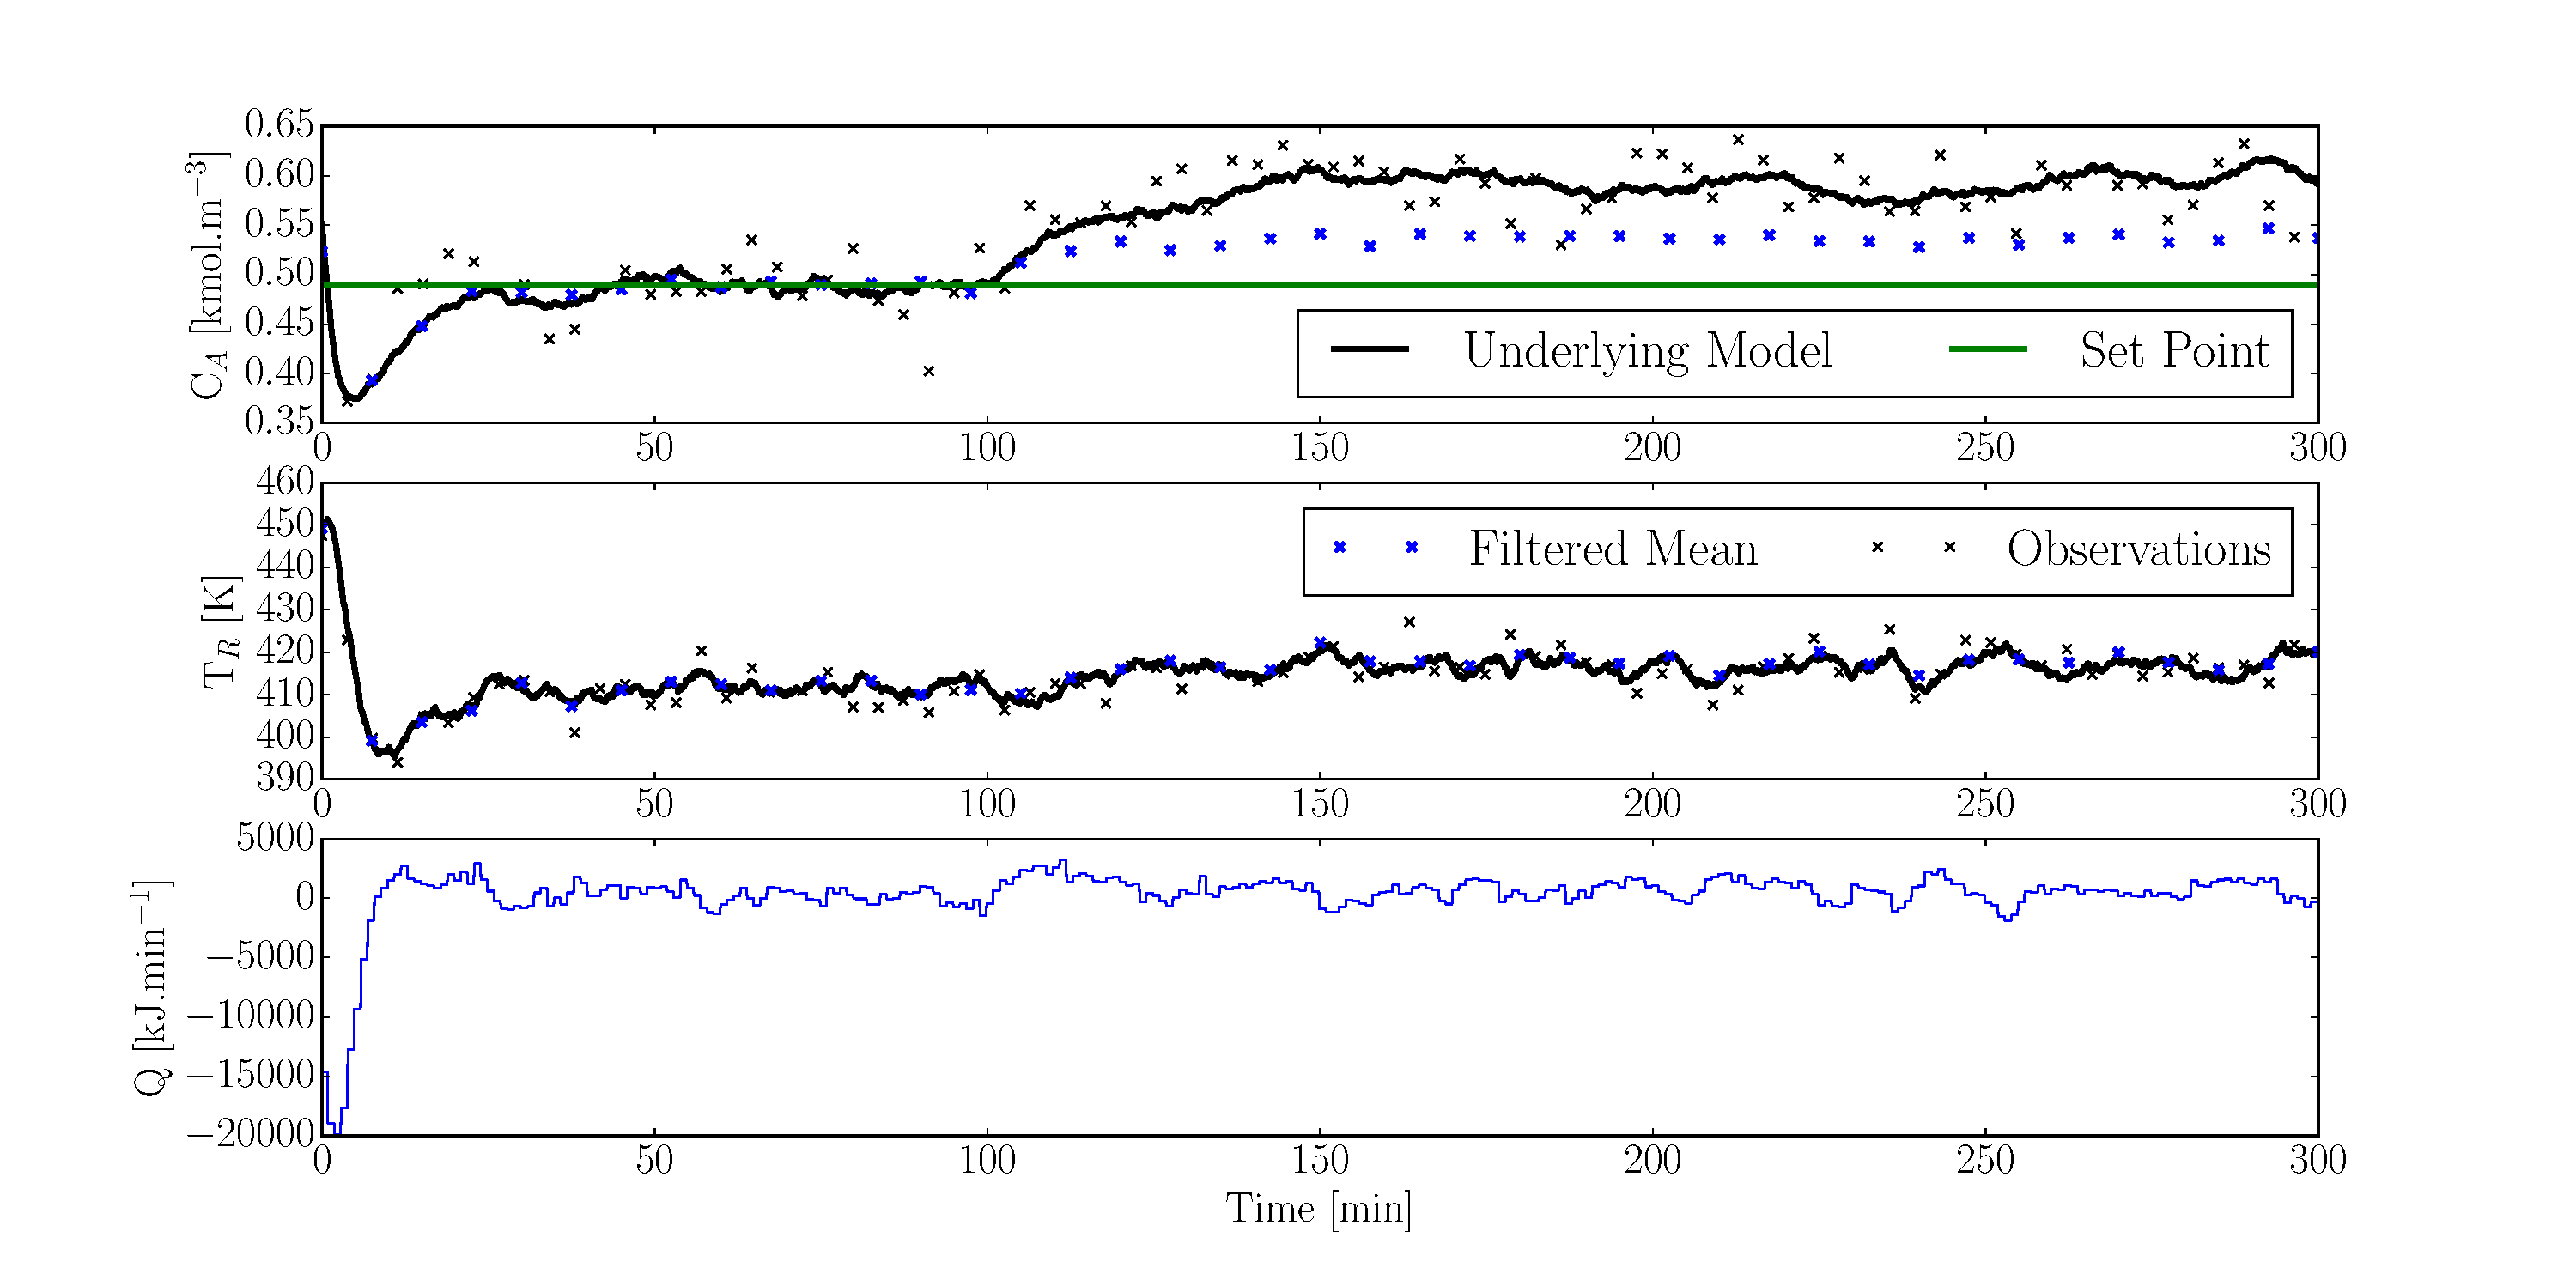
\includegraphics[width=\textwidth]{spf_pf_lqg_track.pdf}
\caption{Standard LQG controller applied to the CSTR where the catalyst denatures at 100 minutes. The bootstrap particle filter was used for inference and the Gaussian approximation of the particles was used.}
\label{fig_spf_pf_lqg_track}
\end{figure}
The average concentration error is 6.79\% and the average controller input is 17.08 kW over the course of the simulation. We can clearly see that there is non-zero set point offset and control is bad in the sense of definition \ref{def_stoch_ref_track_goal}. Clearly the LQG controller is ineffective in this scenario.

We used a constant disturbance model to infer the plant/model mismatch\footnote{The results of this chapter implement the constant disturbance model to achieve zero set point offset. To keep notation the same we do not explicitly show it in (\ref{eq_spf_mpc_expected}) but mention it here.}. This was used to accordingly adjust the controller predictions as discussed in section \ref{sec_switch_mpc_lit}. It is interesting to note that the state estimator infers that the plant reaches set point but in reality there is non-zero offset. This is a consequence of using an inappropriate model in the controller/observer. 

This motivates the use of a controller which intelligently changes the model control is based upon, as discussed previously. In figure \ref{fig_spf_lqg_track} we see the set point tracking ability of the switching controller algorithm using the LQG controller. We have used the switching transition matrix $P_1=\begin{pmatrix}
0.99 & 0.01 \\ 0.01 & 0.99
\end{pmatrix}$ as in section \ref{sec_spf_filtering}.
\begin{figure}[H] 
\centering
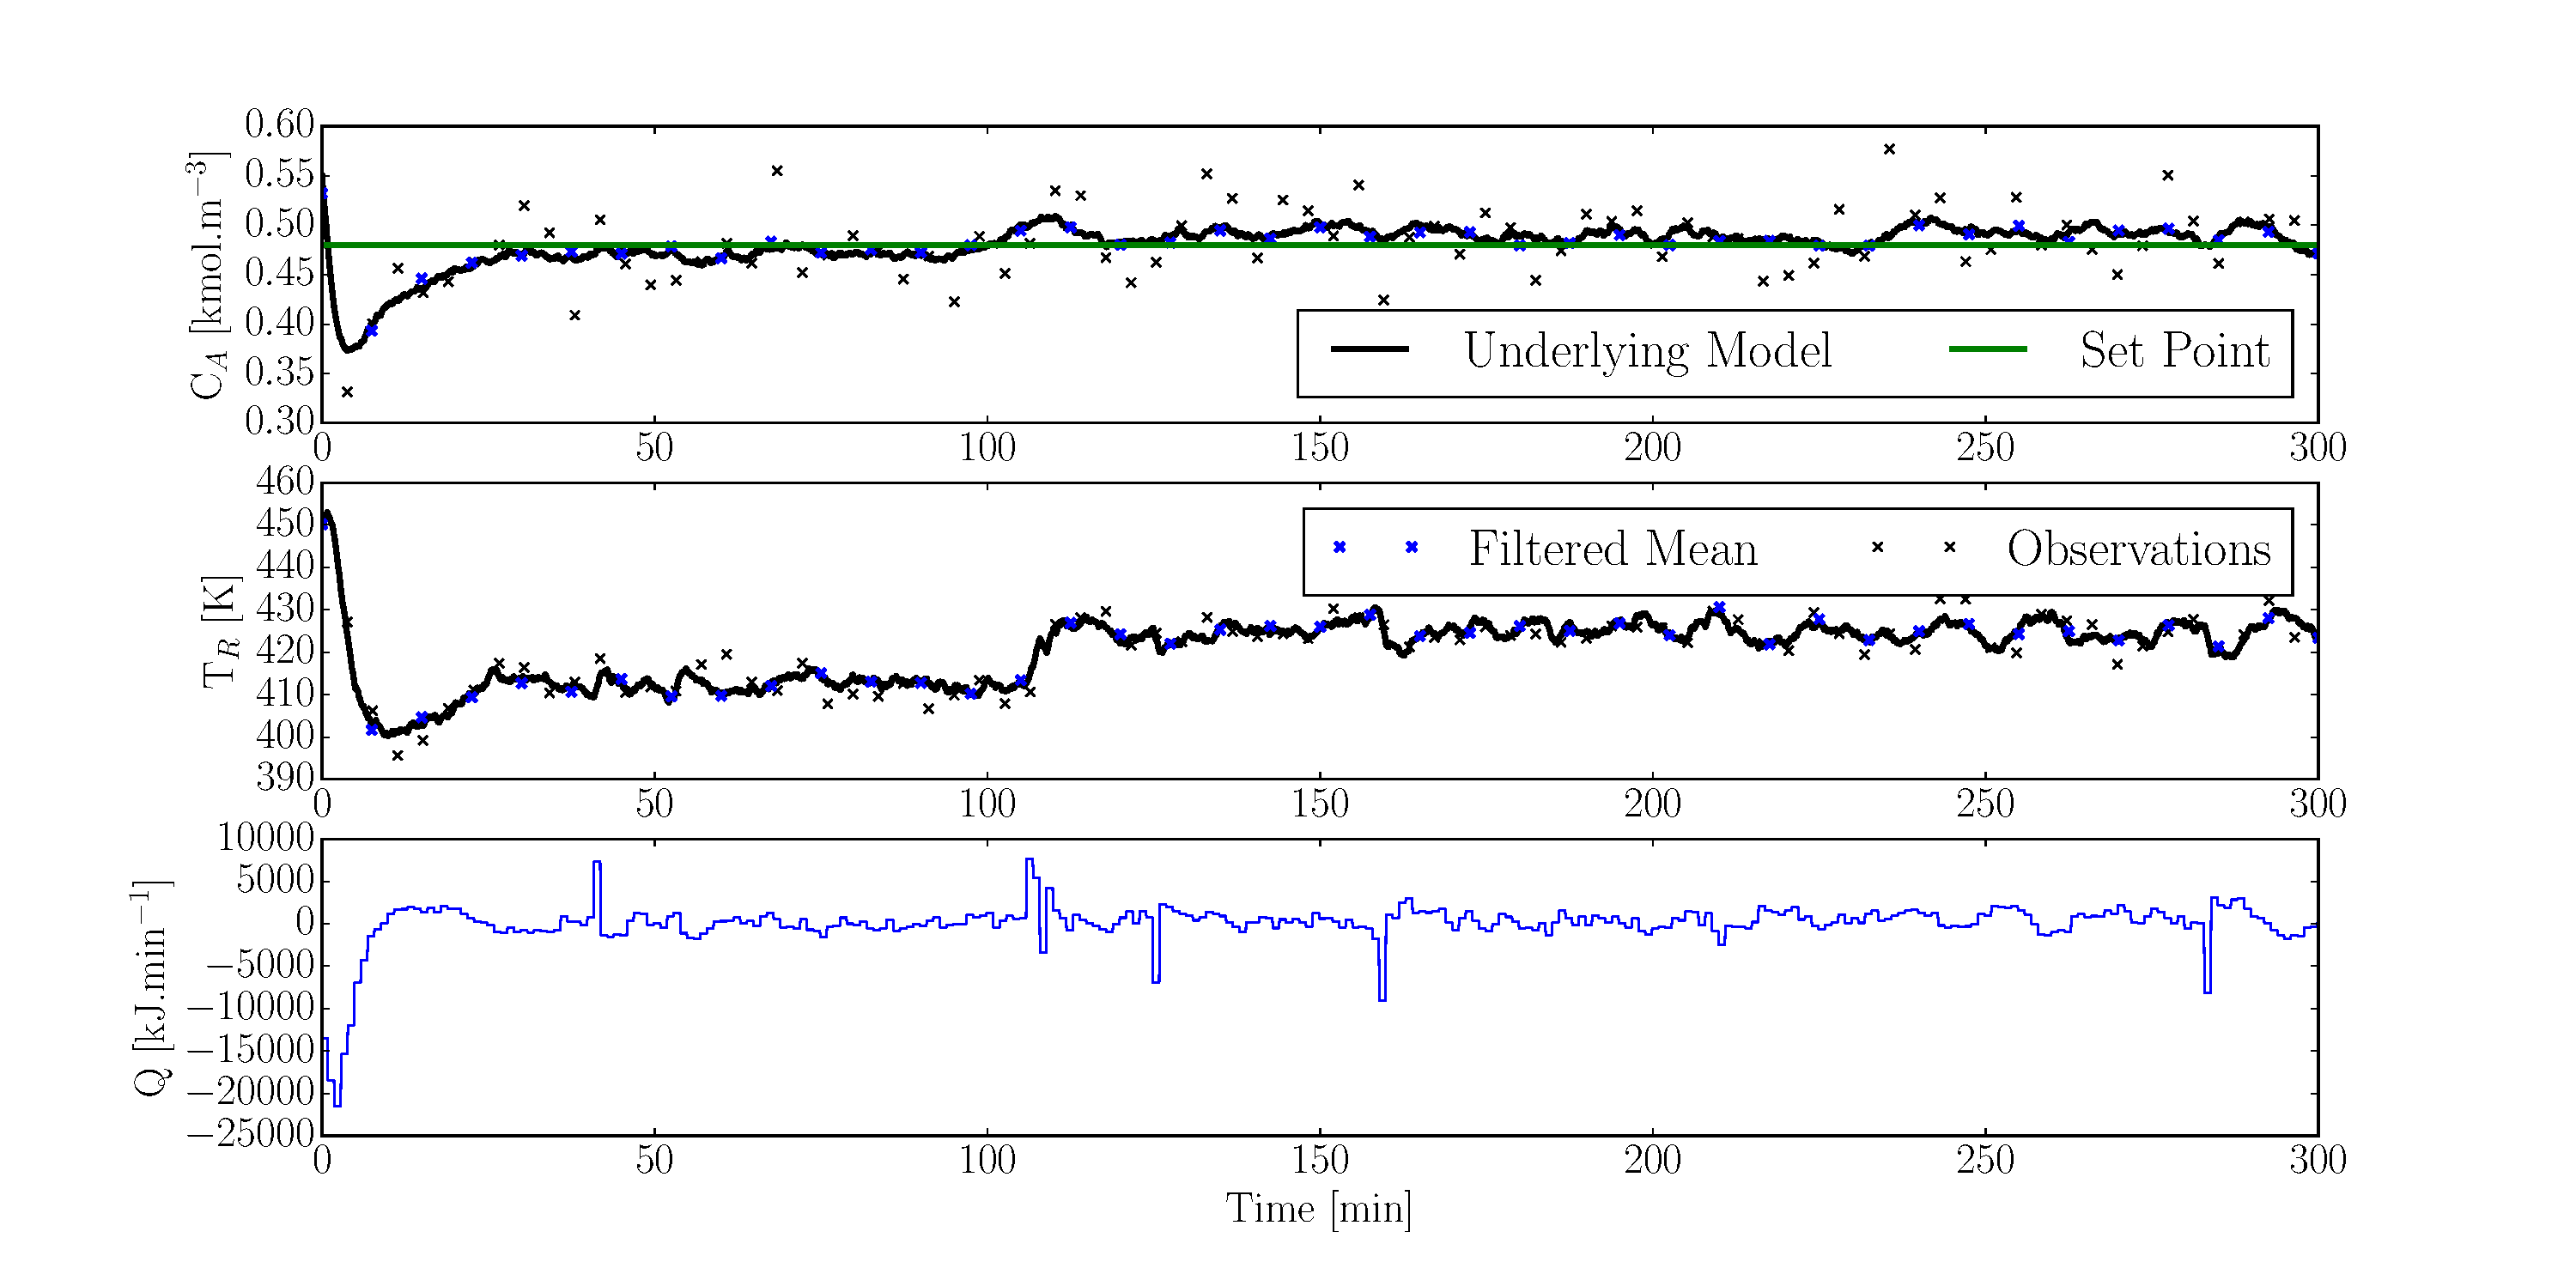
\includegraphics[width=\textwidth]{spf_lqg_track.pdf}
\caption{Switching LQG controller applied to the CSTR where the catalyst denatures at 100 minutes.}
\label{fig_spf_lqg_track}
\end{figure}
The average concentration error is 2.77\% and the average controller input is 28.07 kW. It is clear that we have set point tracking even after the catalyst denatures. By inspecting figure~\ref{fig_spf_lqg_switch} we see that this is not surprising: the filter correctly (for the most part) identifies when the underlying model changes and then uses the better model for control. 
\begin{figure}[H] 
\centering
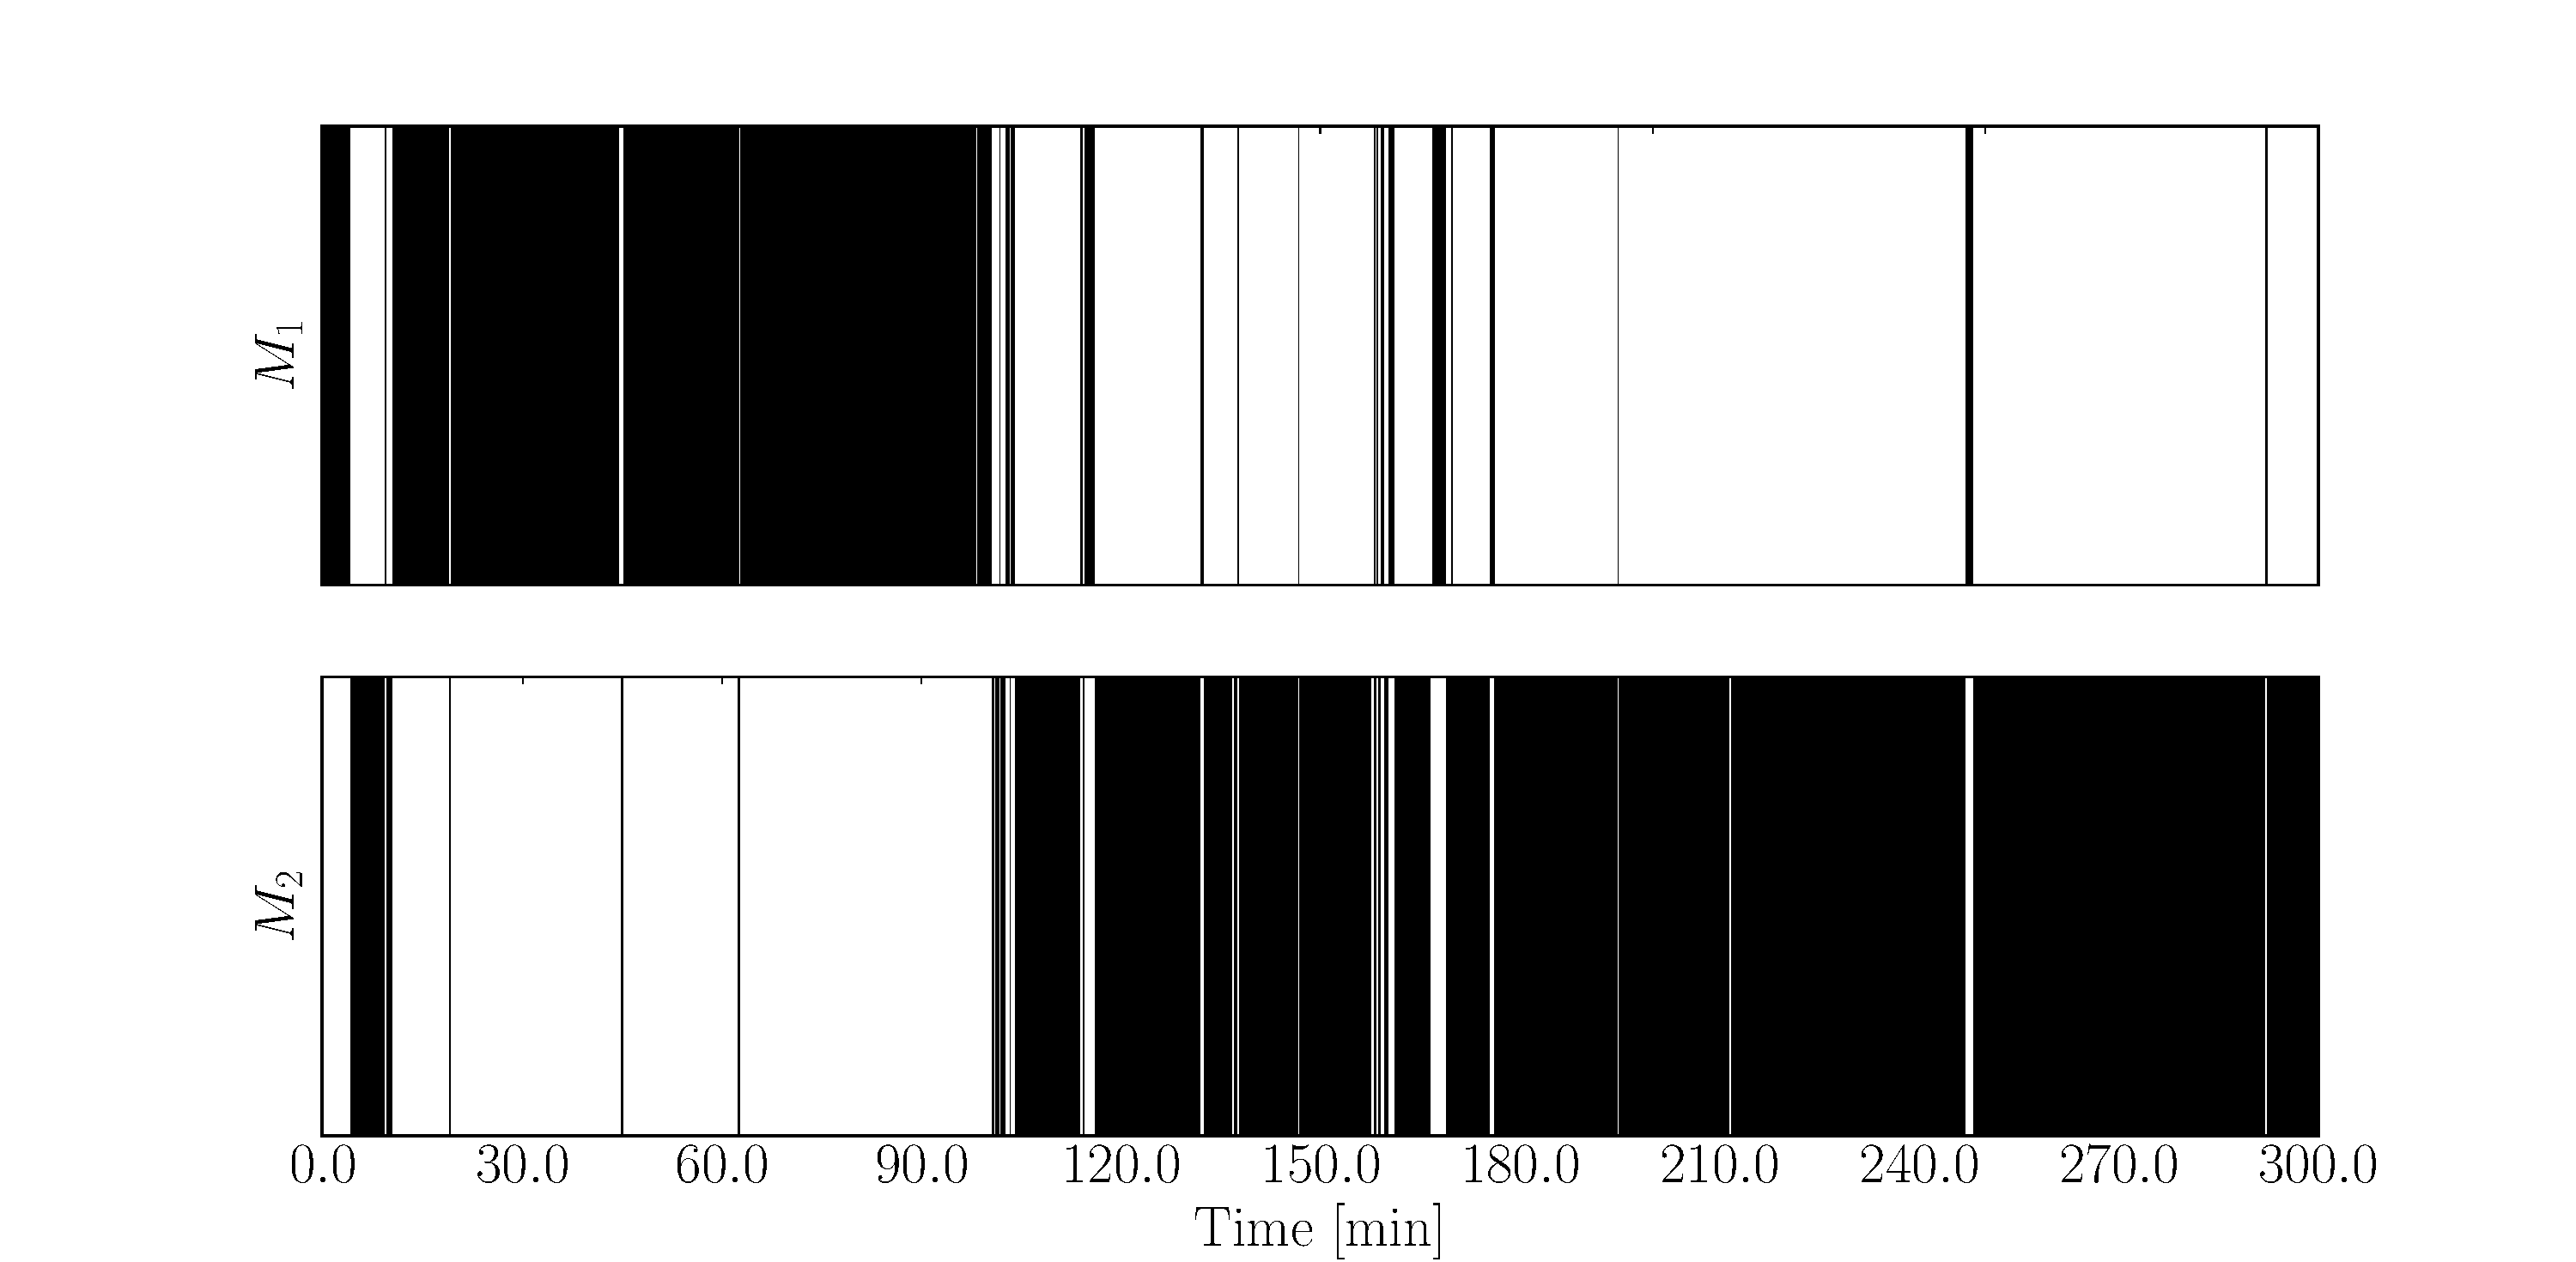
\includegraphics[width=\textwidth]{spf_lqg_switch.pdf}
\caption{Most likely model identified using the particle filter within the context of the switching LQG controller algorithm.}
\label{fig_spf_lqg_switch}
\end{figure}
However, like in sections \ref{sec_rbpf_control_uncon} and \ref{sec_spf_filtering} we see that there is some switching noise. The consequence of this noise is spikes in controller input. This happens because the controller uses the incorrect model to calculate the controller input. In chapter \ref{sec_inf_lin_hybrid} this problem was attenuated by making the switch transition matrix stickier. 

In figures \ref{fig_spf_lqg_track2} and \ref{fig_spf_lqg_switch2} we use exactly the same algorithm except that we have modified the switch transition matrix: $P_2=\begin{pmatrix}
0.999 & 0.001 \\ 0.001 & 0.999
\end{pmatrix}$. Based on figure \ref{fig_spf_lqg_track2} it is clear that we have set point tracking even after the catalyst denatures.
\begin{figure}[H] 
\centering
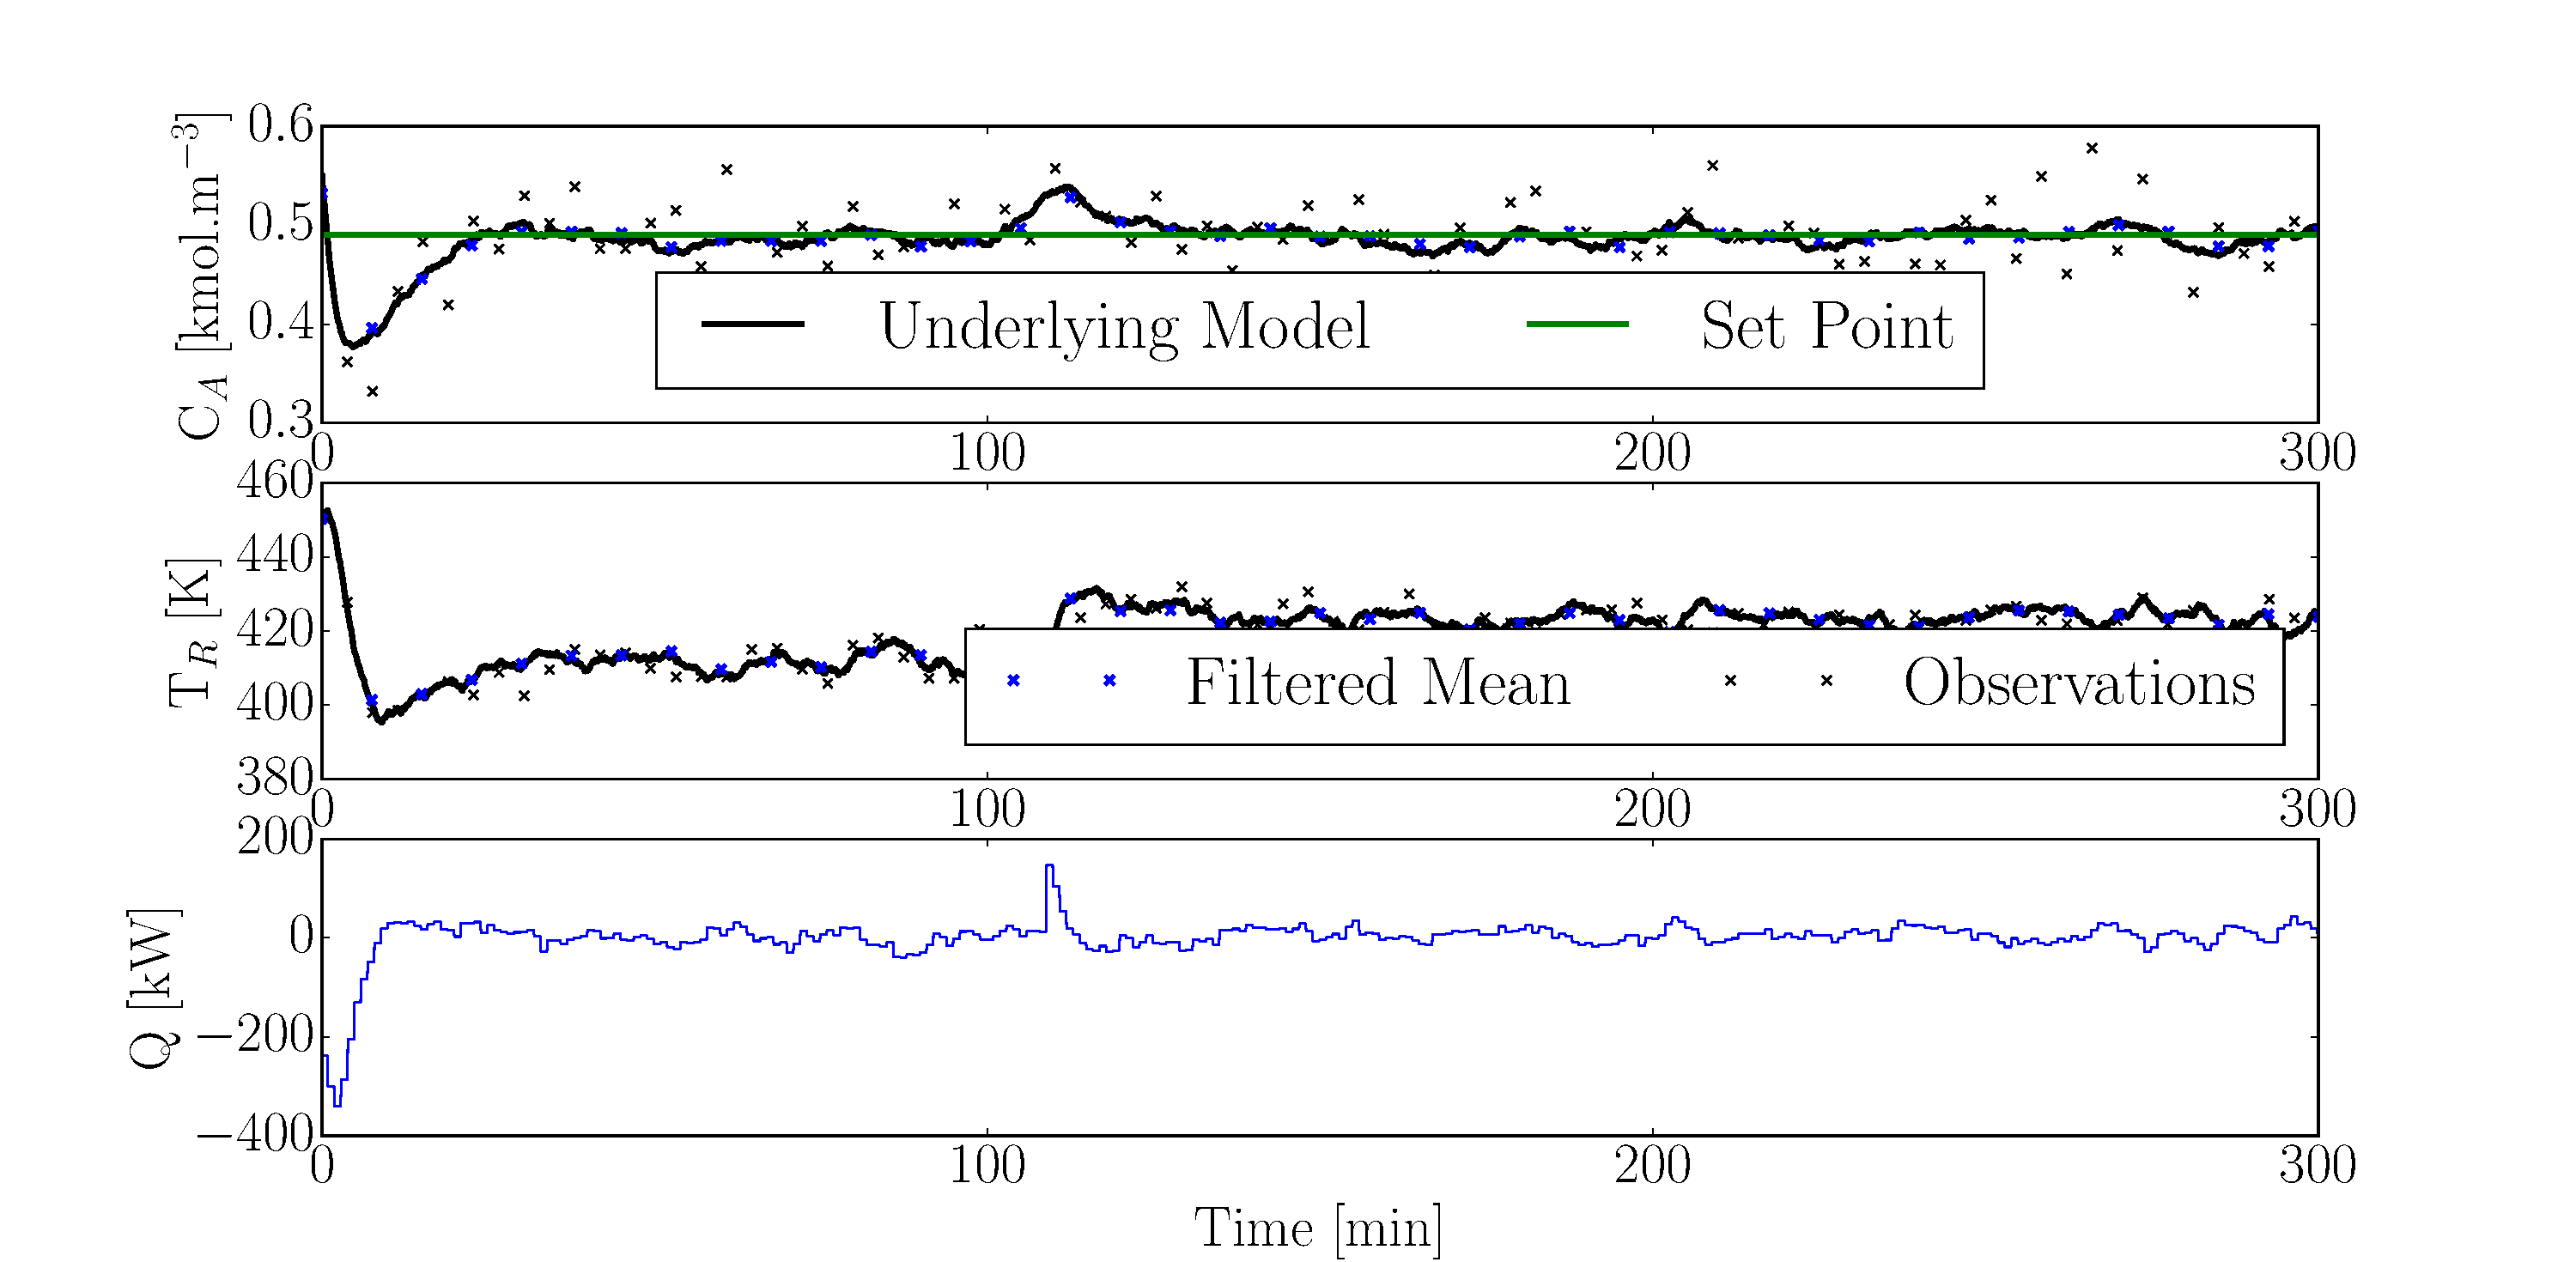
\includegraphics[width=\textwidth]{spf_lqg_track2.pdf}
\caption{Switching LQG controller applied to the CSTR where the catalyst denatures at 100 minutes. Switch transition matrix $P_2$ was used.}
\label{fig_spf_lqg_track2}
\end{figure}
The average concentration error is 2.38\% and the average controller input is 19.06 kW. It is not surprising that the controller, using $P_2$ outperformed the controller using $P_1$. By inspecting figure \ref{fig_spf_lqg_switch2} we see that there is significantly less switcing noise.  
\begin{figure}[H] 
\centering
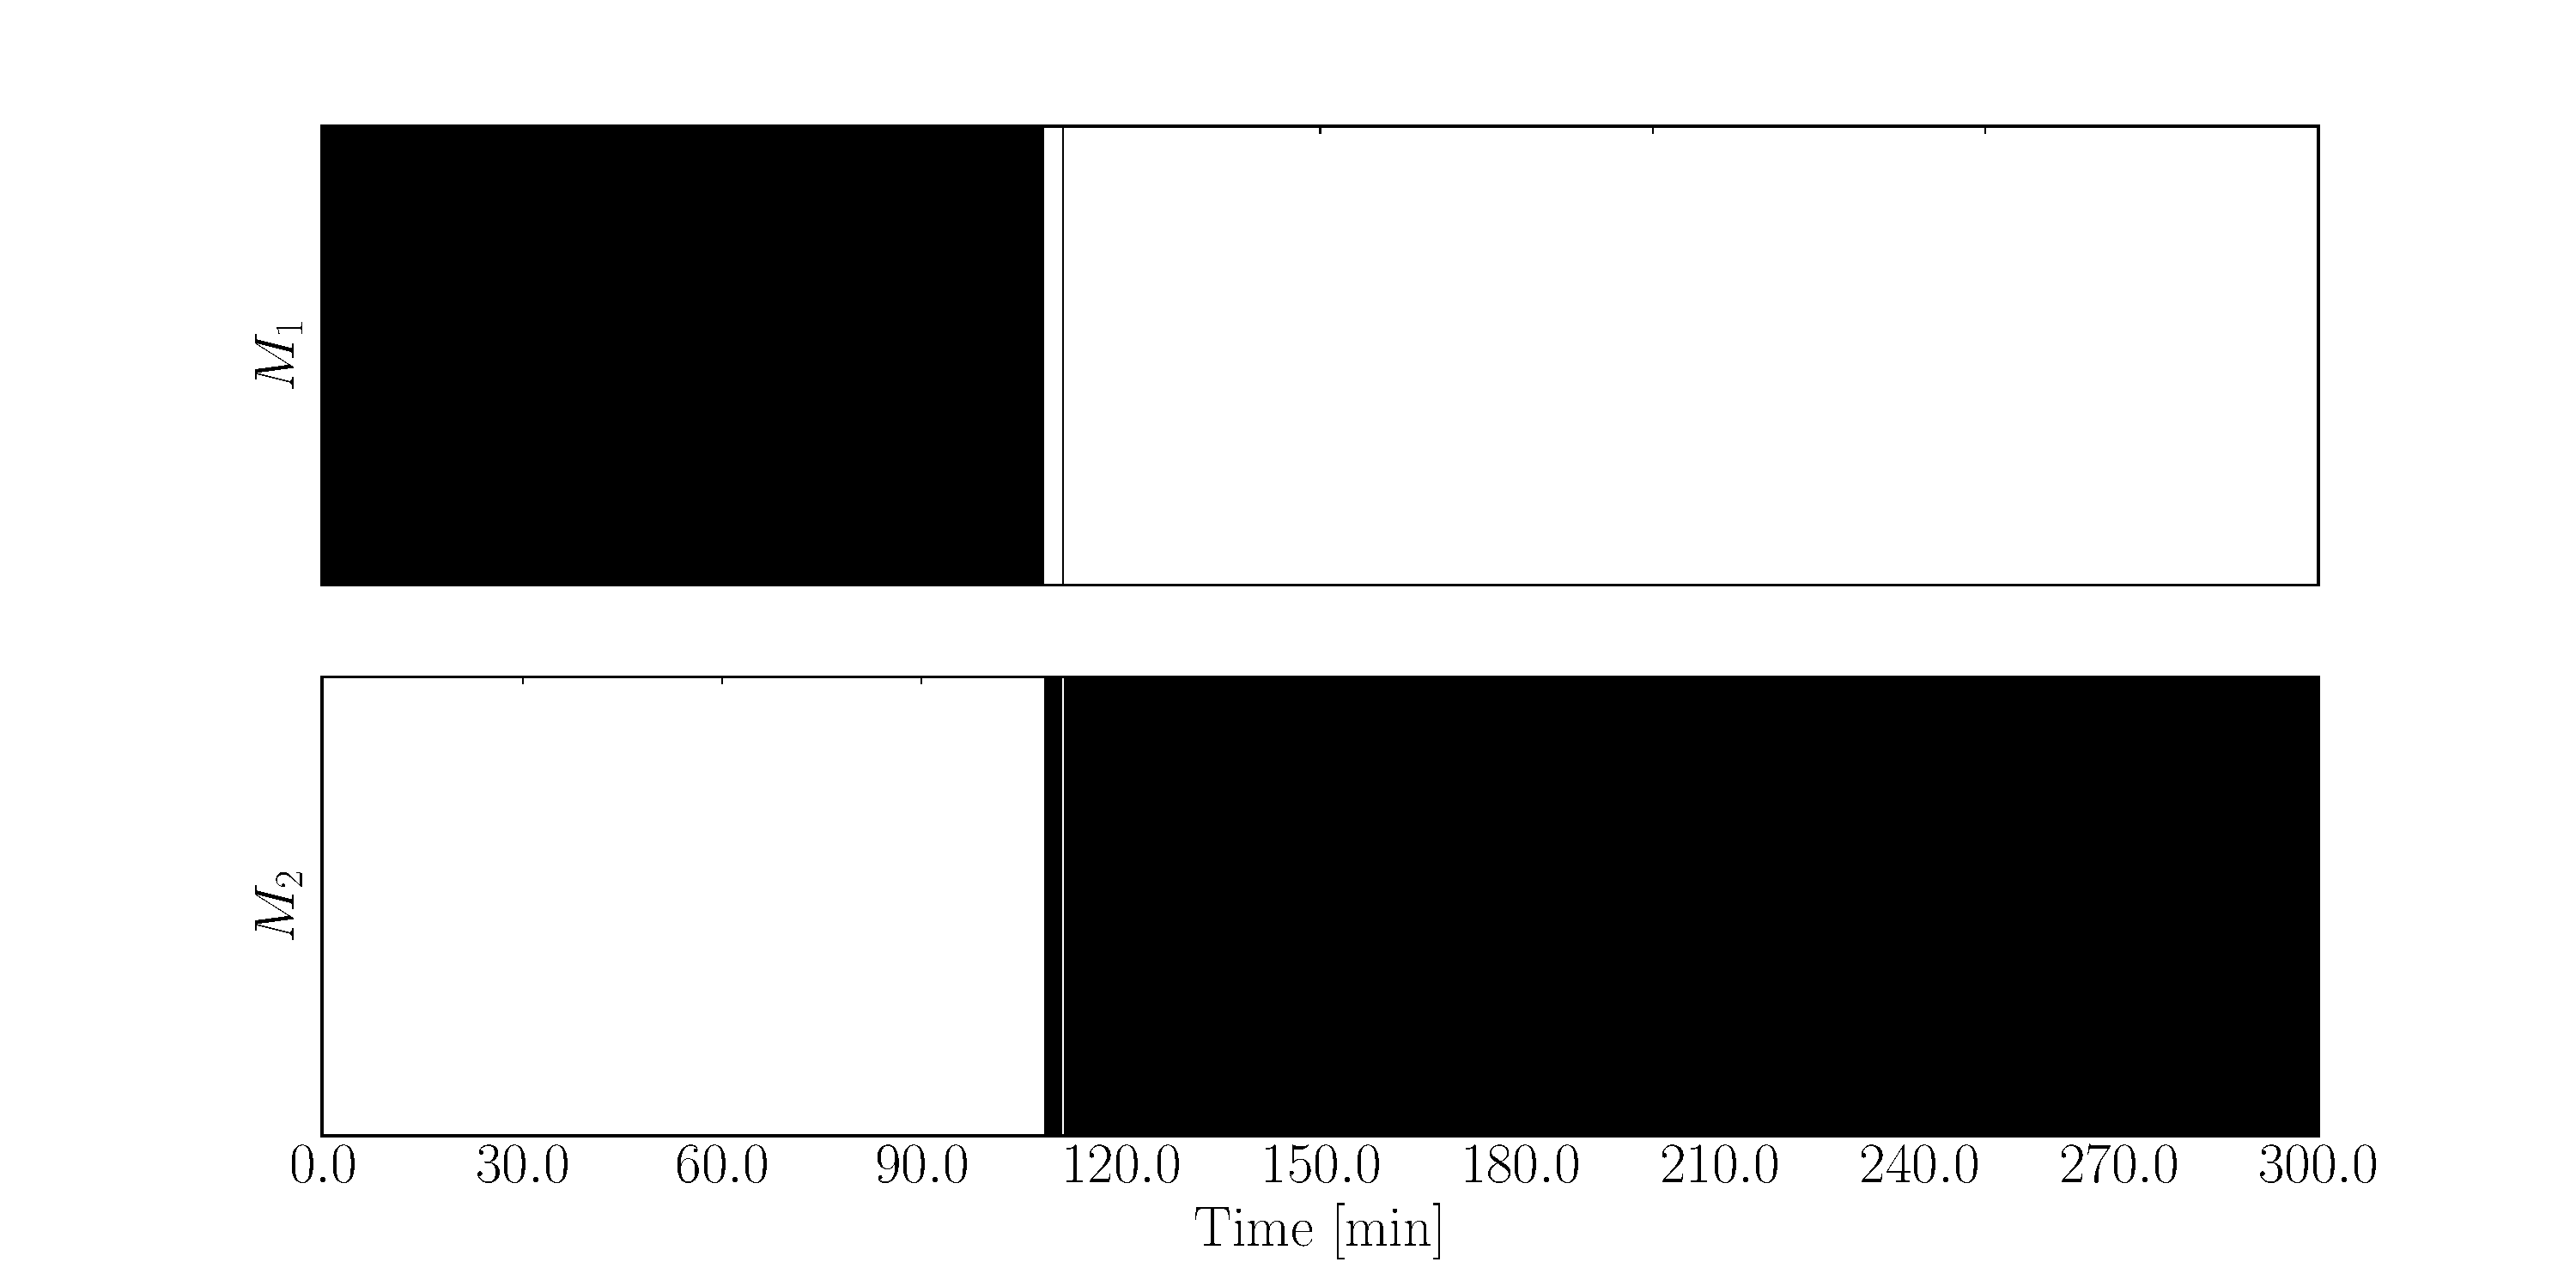
\includegraphics[width=\textwidth]{spf_lqg_switch2.pdf}
\caption{Most likely model identified using the particle filter within the context of the switching LQG controller algorithm. Switch transition matrix $P_2$ was used.}
\label{fig_spf_lqg_switch2}
\end{figure}
Since there is less switching noise there are less controller spikes in figure \ref{fig_spf_lqg_track2} and thus less controller energy is wasted. Finally, a Monte Carlo simulation was performed (using 50 runs) to illustrate that the switching controller works as desired for not just the realisations shown in this chapter. The Monte Carlo absolute average concentration error from set point was 1.30\% taken over the last 10 minutes of each simulation. This indicates that the controller works as desired. We defer further Monte Carlo analysis to the next section.

The results here lend further credibility to our claim that the instability seen in chapter \ref{sec_rbpf_control} is rooted in the inappropriateness of the model used for prediction rather than the switching noise. Figure \ref{fig_spf_lqg_switch} had significant switching noise yet the controller was not unstable. While reducing the amount of switching noise certainly improved control, as figure \ref{fig_spf_lqg_track2} shows, fundamentally we are not using an inappropriate model for control prediction. This difference is was causes the significantly better stability properties seen here.

Motivated by the success of the switching LQG controller we incorporate constraints in the sequel.

\section{Constrained switching control} 
In this section we extend the switching controller algorithm of section \ref{sec_spf_uncon} to the deterministic and stochastic MPCs introduced in section \ref{sec_lin_mpc_constained}. We use the same parameters as before. Like in section \ref{sec_lin_sys_cont} we first illustrate the performance of the stochastic MPC controller with expected value constraints,
\begin{equation}
\begin{aligned}
&\underset{\mathbf{u}}{\text{min }} \mathbb{E}\left[ \frac{1}{2}\sum_{k=0}^{N-1} \left( x_k^TQx_k + u_k^TRu_k \right) + \frac{1}{2}x_N^TP_fx_N \right] \\
& \text{subject to } x_{t+1}=A_ix_t+B_iu_t + w_t\\
& \text{and } \mathbb{E}[\begin{pmatrix}
10 \\ 1
\end{pmatrix}^Tx_t + 400] \geq 0 ~\forall ~t=1,...,N \\
& \text{and } |u_t| \leq 250 ~\forall ~t=0,...,N-1,
\end{aligned}
\label{eq_spf_mpc_expected}
\end{equation} 
(for some model $M_i$) and then incorporate chance constraints later. Using the results of section \ref{sec_lin_mpc_constained} we know that (\ref{eq_spf_mpc_expected}) can be reformulated as a deterministic problem given the (Gaussian) current state estimate $x_0$. The state estimate is derived from either the particle filter or switching particle filter using 200 and 500 particles respectively. For the switching particle filter we use the switch transition matrix $P_2$ due to the results in section \ref{sec_spf_uncon}.

In figure \ref{fig_spf_pf_mpc_track} we see the set point tracking performance of (\ref{eq_spf_mpc_expected}) using the same particle filter as used in section \ref{sec_spf_uncon}. Since the particle filter only uses the healthy plant model we only use $M_1$. 
\begin{figure}[H] 
\centering
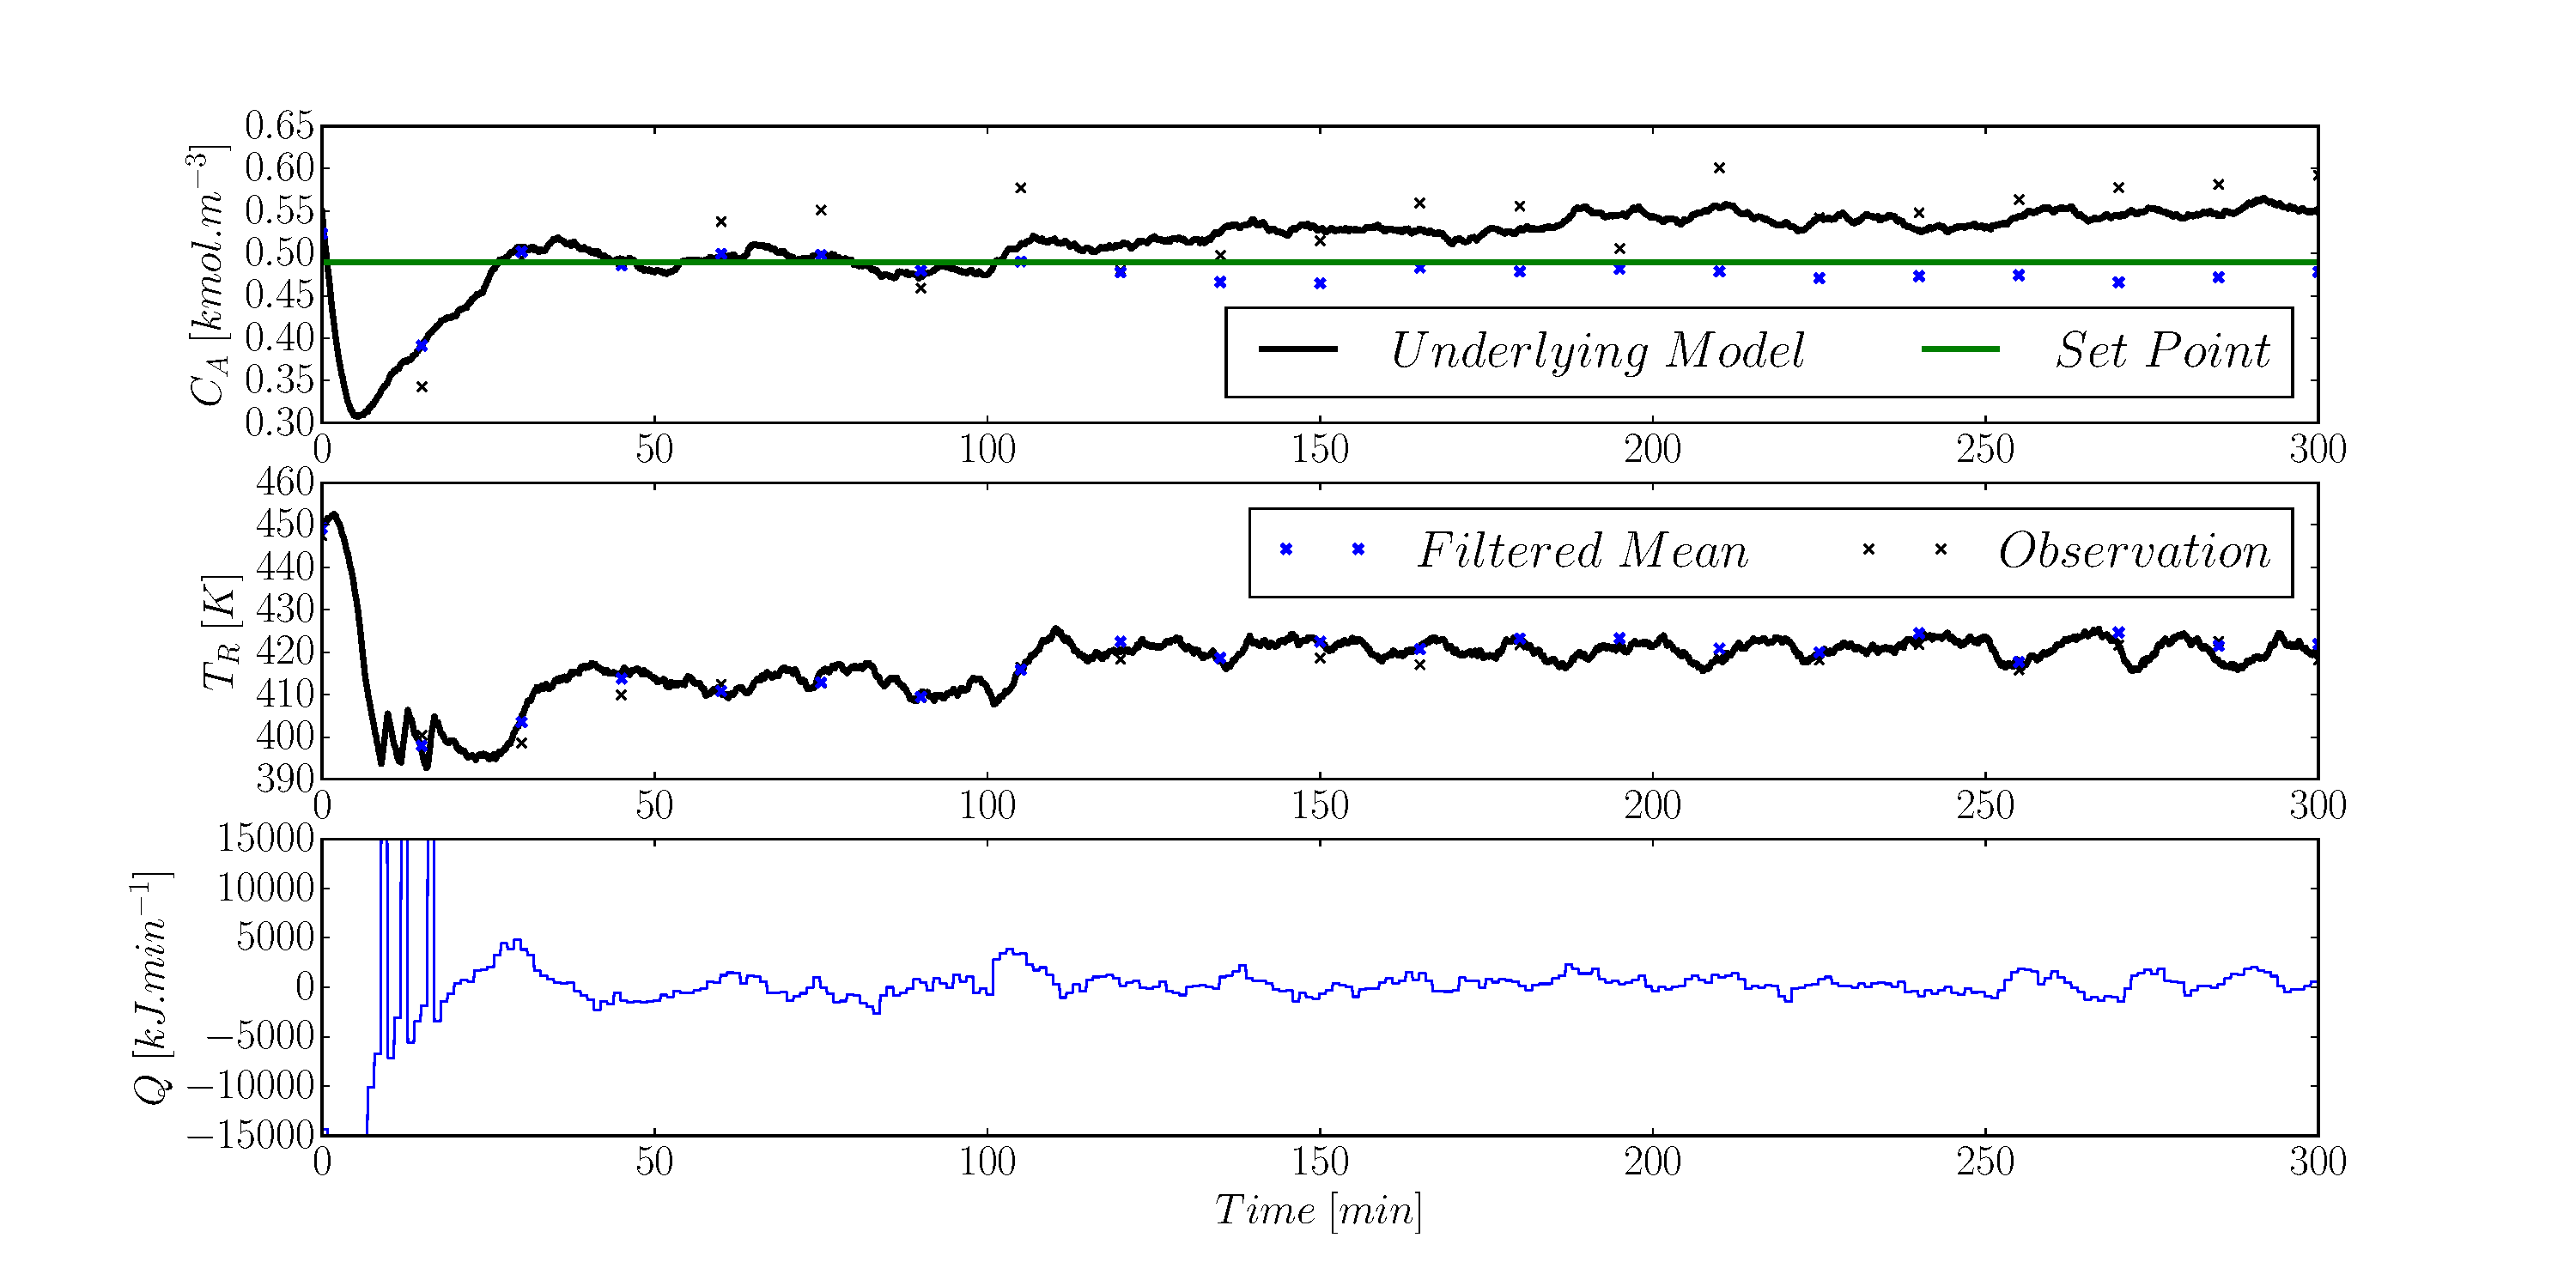
\includegraphics[width=\textwidth]{spf_pf_mpc_track.pdf}
\caption{Deterministic MPC using a particle filter as the state estimator. The initial point is $(0.55, 450)$. An integrating disturbance model was used to estimate the mismatch between the underlying system and the controller model. The catalyst denatures at 100 minutes.}
\label{fig_spf_pf_mpc_track}
\end{figure}
The average concentration error is 8.33\% and the average controller input is 24.21 kW. Unfortunately we do not observe zero set point offset control but rather zero offset state estimates. Clearly the controller input generated by the MPC, which is based on the healthy plant, only drives the particle filter's predictions to the set point. We can see that the classic disturbance model approach \cite{lee} to ensure zero set point offset fails here because the underlying (faulty) model is too different from the controller model. Intuitively, we are attempting to control a tricycle (the faulty plant) using a model of a Ferrari.  

In figure \ref{fig_spf_mpc_track} we see the switching controller algorithm applied within the context of (\ref{eq_spf_mpc_expected}). The model corresponding to the highest weighted switch at each time step was selected for control.
\begin{figure}[H] 
\centering
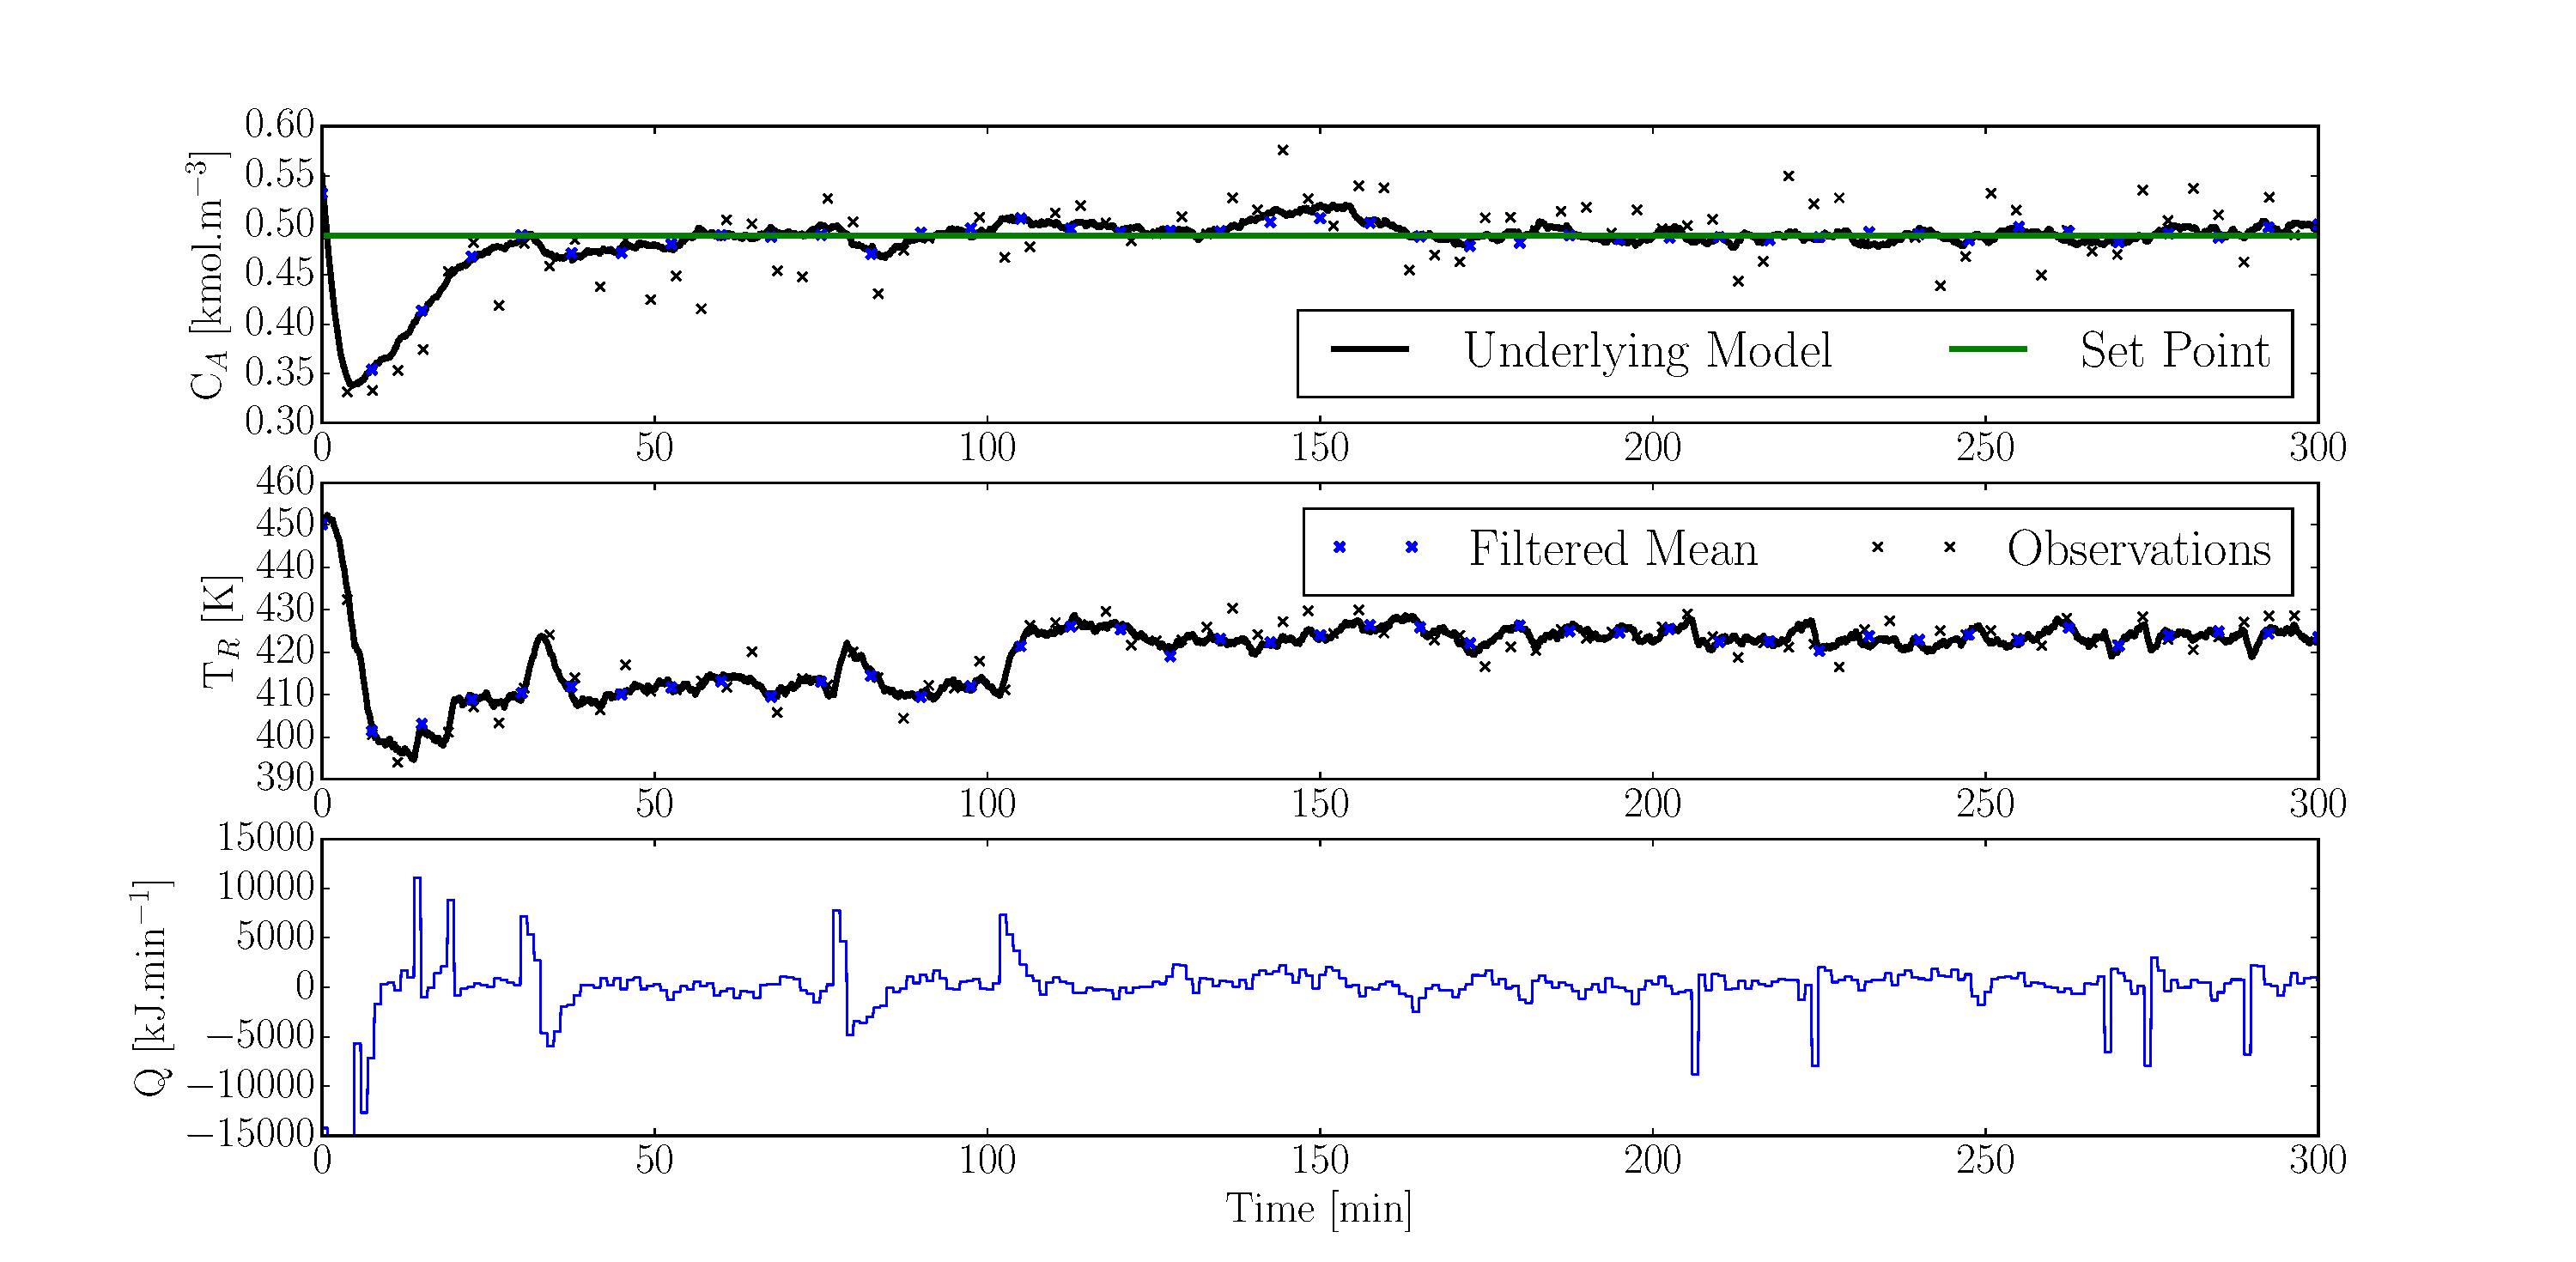
\includegraphics[width=\textwidth]{spf_mpc_track.pdf}
\caption{The switching MPC controller algorithm applied to the CSTR with catalyst which denatures at 100 minutes.}
\label{fig_spf_mpc_track}
\end{figure}
The average concentration error is 3.19\% and the average controller input is 22.61 kW over the simulation time span. The performance of the switching controller is significantly better than the non-switching case. This is not surprising because, as figure \ref{fig_spf_mpc_switch} shows, the filter correctly identifies when the plant breaks. The tell tale controller spike is also evident after 100 minutes indicating that the controller switched.
\begin{figure}[H] 
\centering
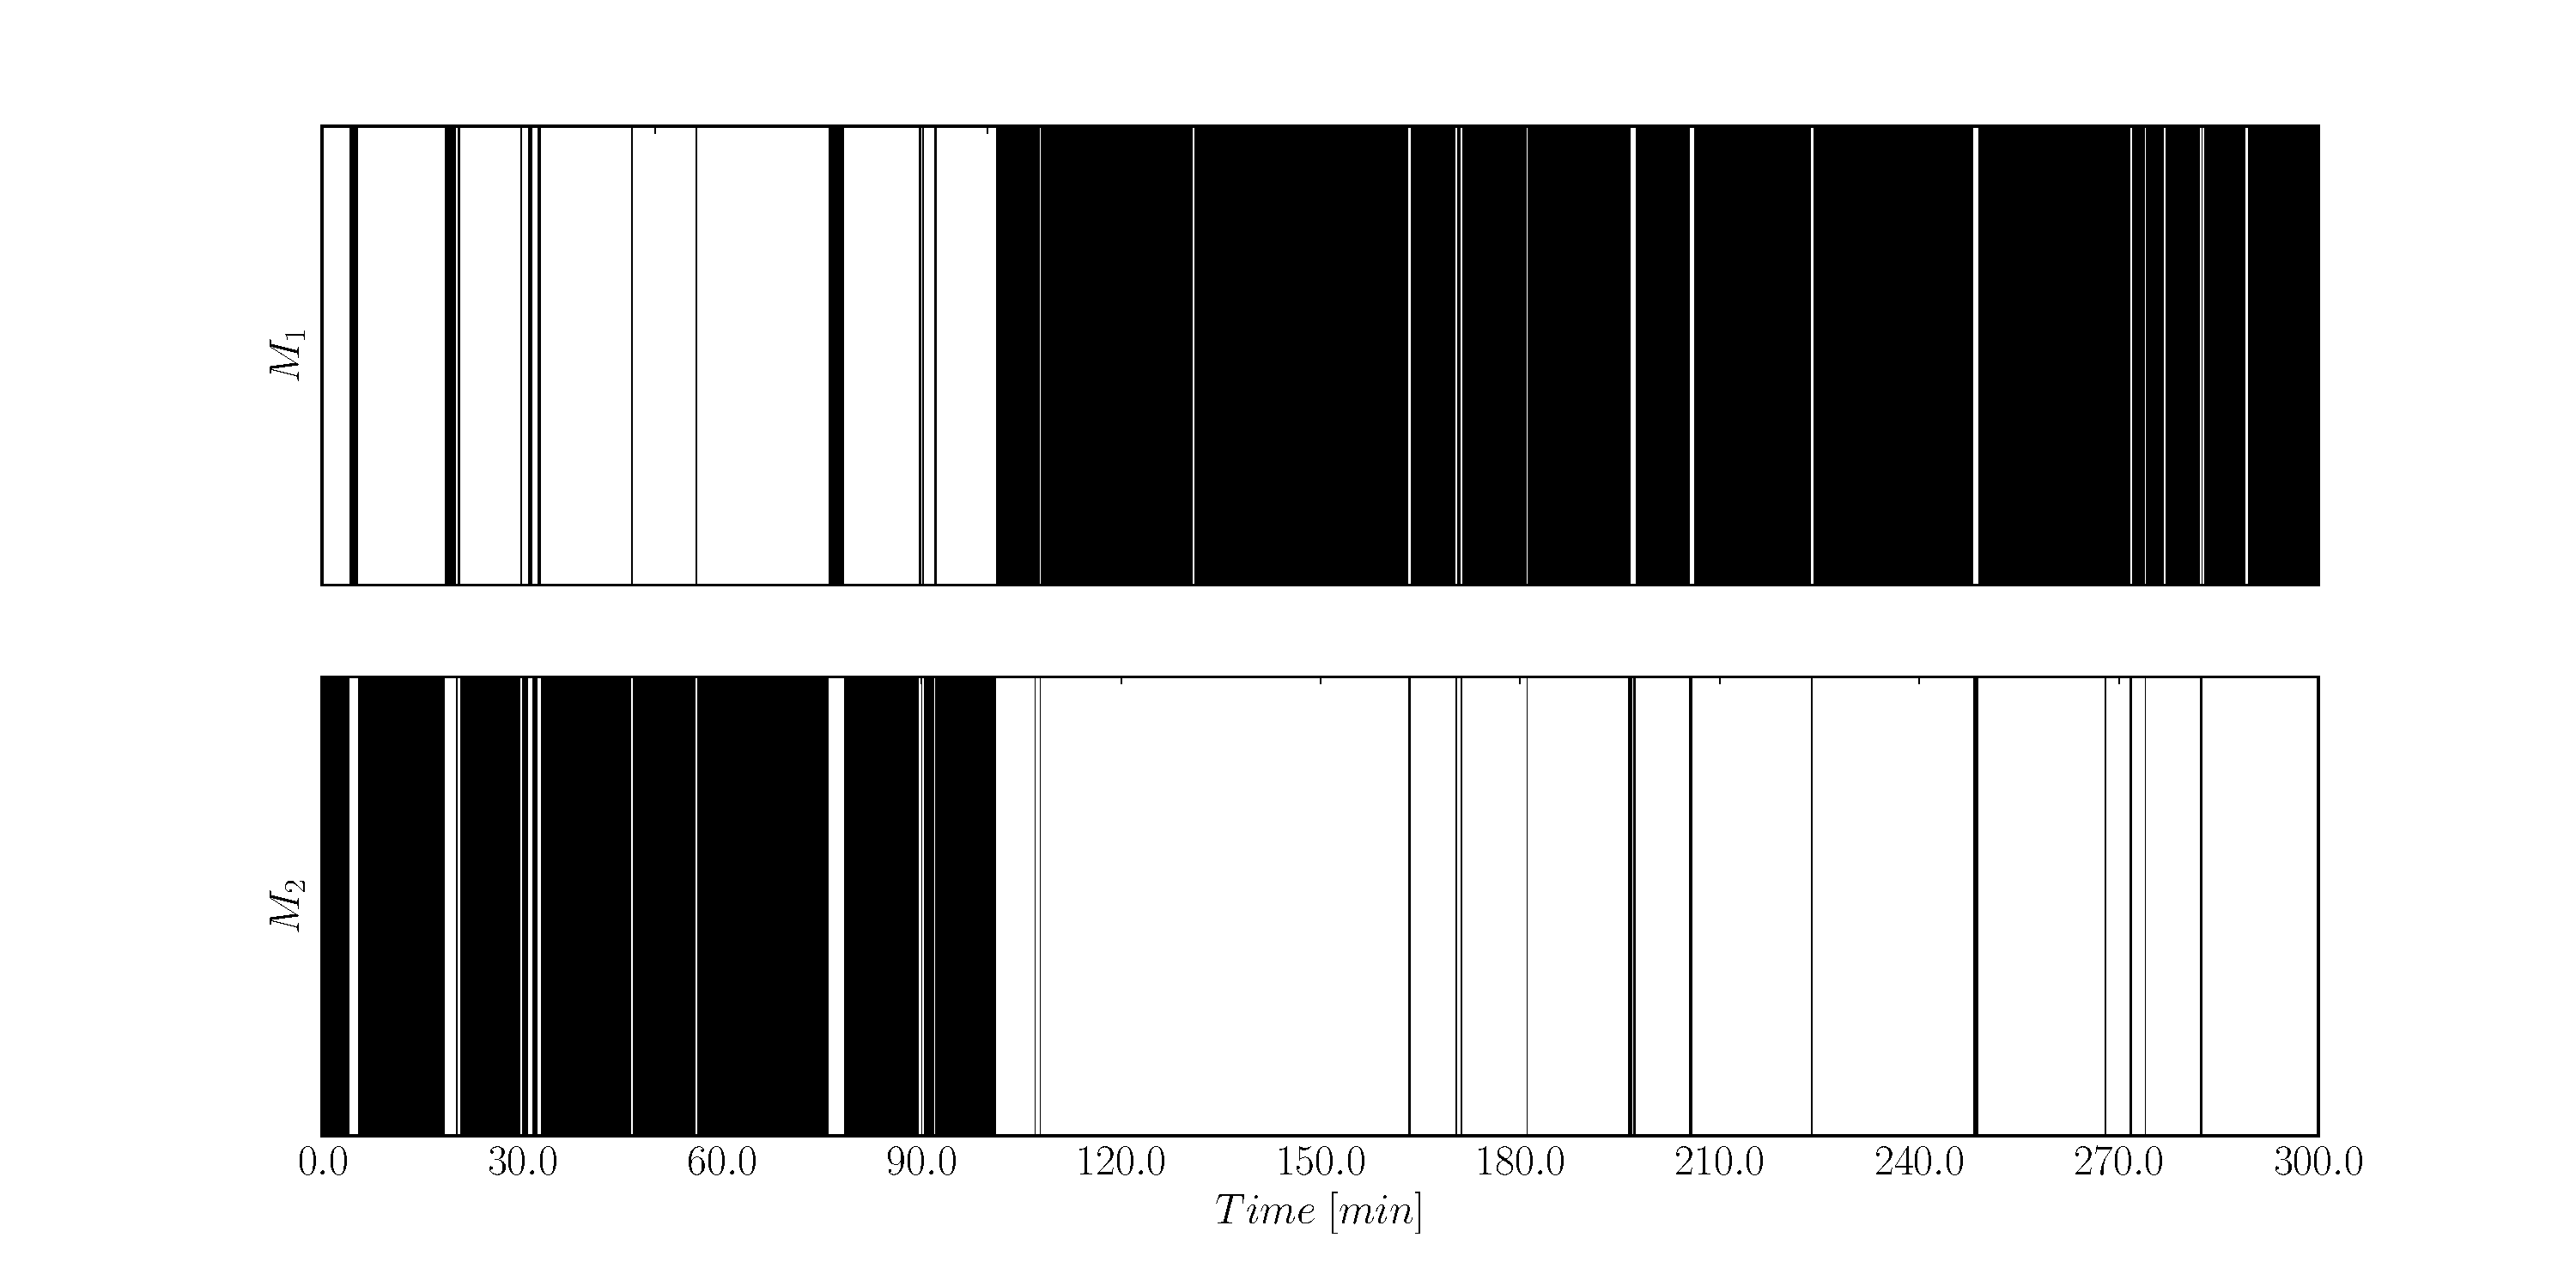
\includegraphics[width=\textwidth]{spf_mpc_switch.pdf}
\caption{Most likely model identified using the particle filter within the context of the switching MPC controller algorithm.}
\label{fig_spf_mpc_switch}
\end{figure}
There is almost no switching noise in figure \ref{fig_spf_lqg_switch} due to the static nature of the switch transition matrix $P_2$. If $P_1$ were used we would expect more noise. As mentioned in chapter~\ref{sec_inf_lin_hybrid} switching noise is not necessarily bad for inference. We do see that the filter does not immediately notice that the underlying model has changed. The stickier the switch transition matrix is the longer it will take for the controller to adjust the model. Depending on the application this delay could be problematic. On the other hand, the switching noise causes controller input spikes which could also be bad for control. 

In figure \ref{fig_spf_mpc_state} we see the state space trajectory of the expected value constraint MPC. It is clear that the operating temperature associated with the set point moves when the catalyst denatures.
\begin{figure}[H] 
\centering
\includegraphics[width=\textwidth]{spf_mpc_state.pdf}
\caption{State space trajectory of the expected value constrained stochastic MPC using the switching controller algorithm.}
\label{fig_spf_mpc_state}
\end{figure}
Clearly there is a constraint violation - similar to that found in sections \ref{sec_lin_sys_cont} and \ref{sec_nonlinear_control}. By extending the MPC problem of (\ref{eq_spf_mpc_expected}) to the chance constrained problem 
\begin{equation}
\begin{aligned}
&\underset{\mathbf{u}}{\text{min }} \mathbb{E}\left[ \frac{1}{2}\sum_{k=0}^{N-1} \left( x_k^TQx_k + u_k^TRu_k \right) + \frac{1}{2}x_N^TP_fx_N \right] \\
& \text{subject to } x_{t+1}=A_ix_t+B_iu_t + w_t\\
& \text{and } \mathbb{E}[\begin{pmatrix}
10 \\ 1
\end{pmatrix}^Tx_t + 400] \geq 0 ~\forall ~t=1,...,N \\
& \text{and } \text{Pr}(\begin{pmatrix}
10 \\ 1
\end{pmatrix}^T x_t + 400 \geq 0) \geq 0.99 ~\forall ~t=1,...,N\\
& \text{and } |u_t| \leq 250 ~\forall ~t=0,...,N-1\\
\end{aligned}
\label{eq_spf_mpc_chance}
\end{equation} 
we attempt to ensure that the constraint is not violated in this way. The same switching controller algorithm, as discussed previously, is implemented. We have used the 99\% chance constraint to highlight the effectiveness of the method compared to the expected value version. 

In figure \ref{fig_spf_mpc_track2} we see that the switching chance constrained MPC successfully tracks the set point.
\begin{figure}[H] 
\centering
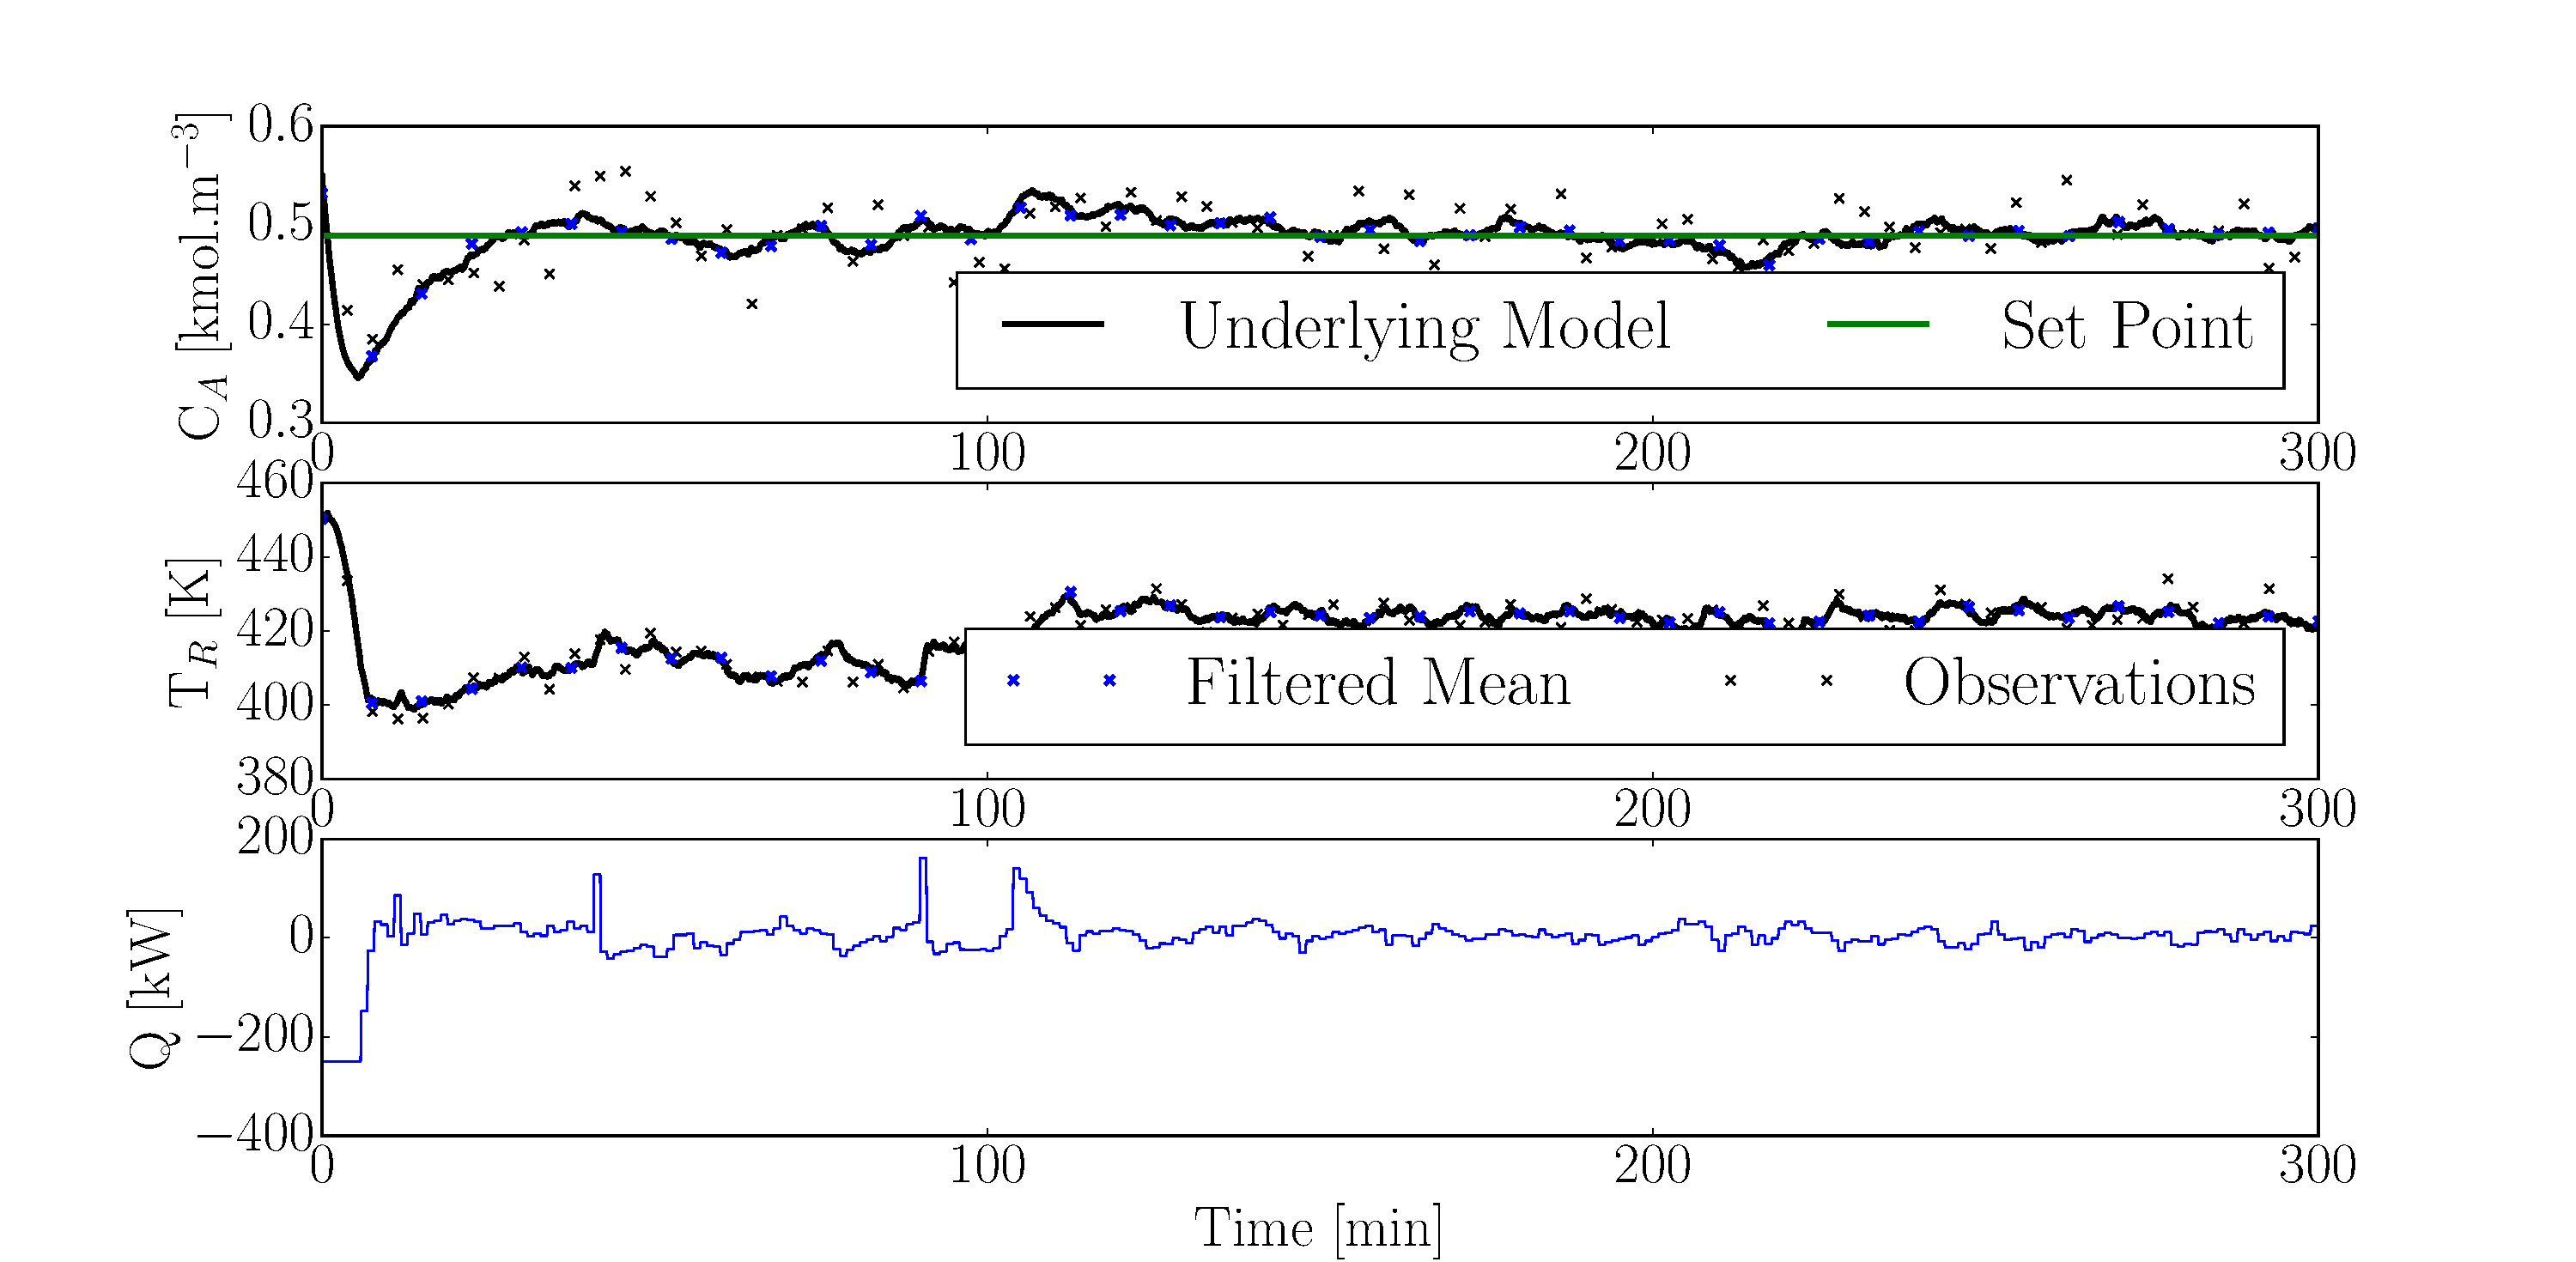
\includegraphics[width=\textwidth]{spf_mpc_track2.pdf}
\caption{The switching MPC controller algorithm applied to the CSTR with catalyst which denatures at 100 minutes. The chance constrained MPC was used.}
\label{fig_spf_mpc_track2}
\end{figure}
The average concentration error is 3.01\% and the average controller input is 22.03 kW. In figure \ref{fig_spf_mpc_switch2} we see the familiar model switching diagram. Clearly the controller isolates when the fault occurs and tracks the set point successfully. 
\begin{figure}[H] 
\centering
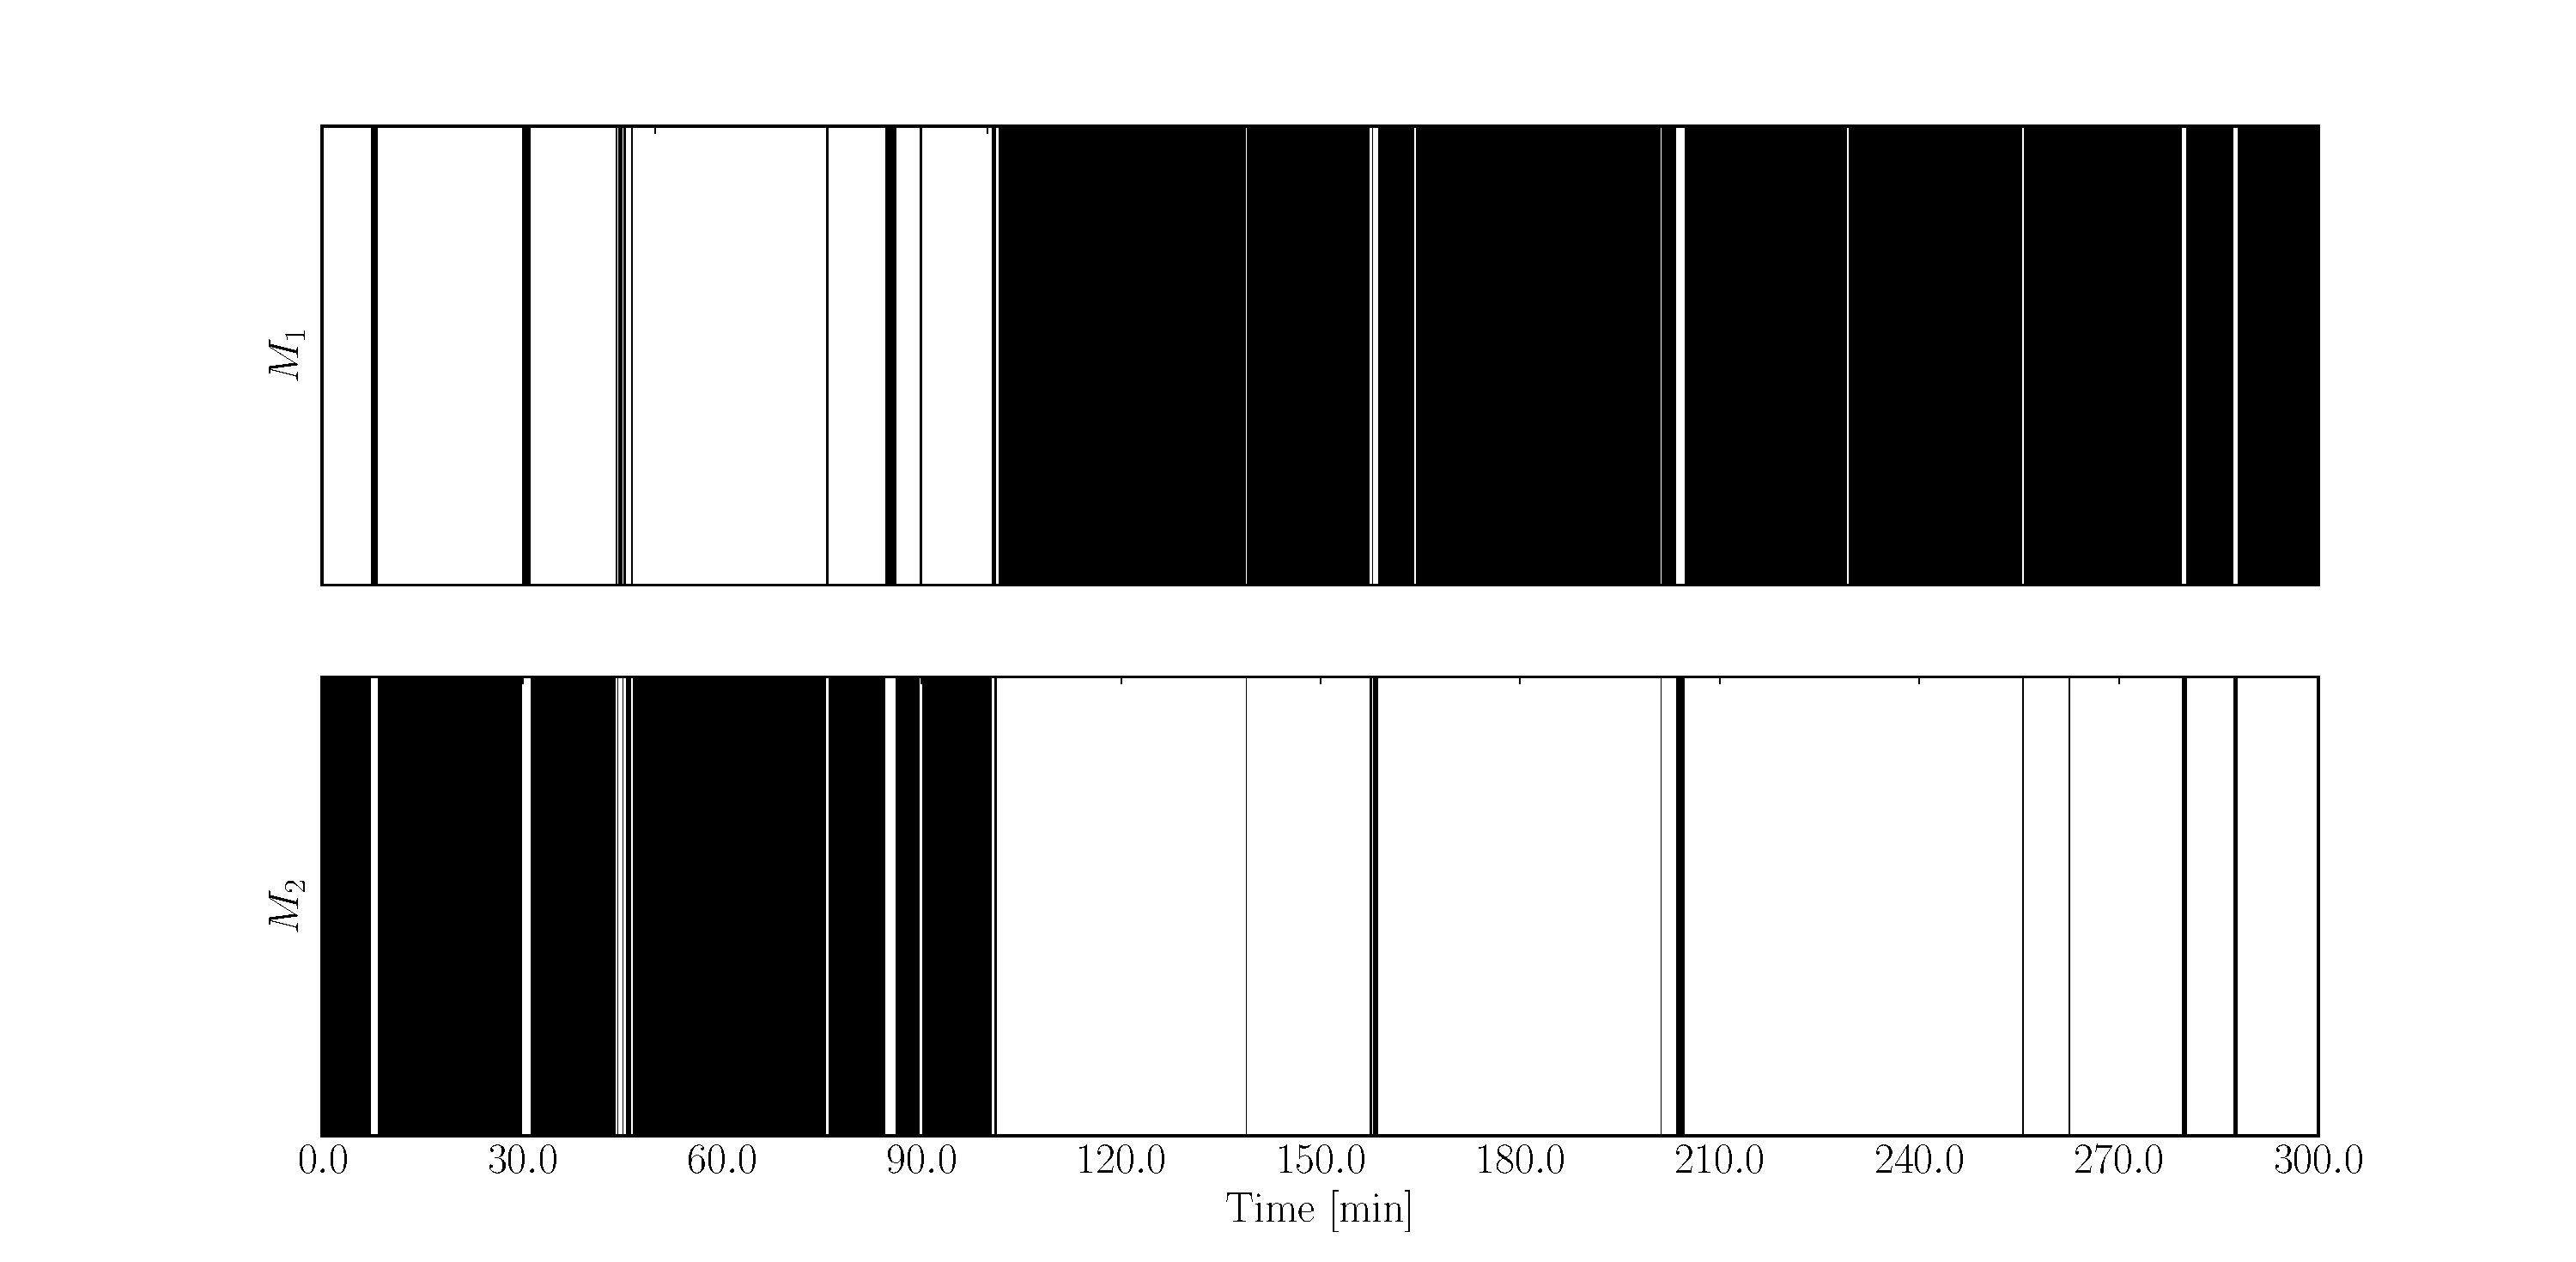
\includegraphics[width=\textwidth]{spf_mpc_switch2.pdf}
\caption{Most likely model identified using the particle filter within the context of the chance constrained switching MPC controller algorithm.}
\label{fig_spf_mpc_switch2}
\end{figure}
Finally, in figure \ref{fig_spf_mpc_state2} we see that the constraint is not violated.
\begin{figure}[H] 
\centering
\includegraphics[width=\textwidth]{spf_mpc_state2.pdf}
\caption{State space trajectory of the chance constrained stochastic MPC using the switching controller algorithm.}
\label{fig_spf_mpc_state2}
\end{figure}
Since figure \ref{fig_spf_mpc_state2} only illustrates that the constraint is not violated for a single run we again use a Monte Carlo technique to justify the assertion that, for this example, the stochastic controller can successfully reduce the constraint violation probability. In figure \ref{fig_spf_mc} we have used the data of over 500 simulations to illustrate the benefit, in terms of constraint violation characteristics, of using the switching controller algorithm with the stochastic MPC controllers developed in chapter \ref{sec_linear_control}.
\begin{figure}[H] 
\centering
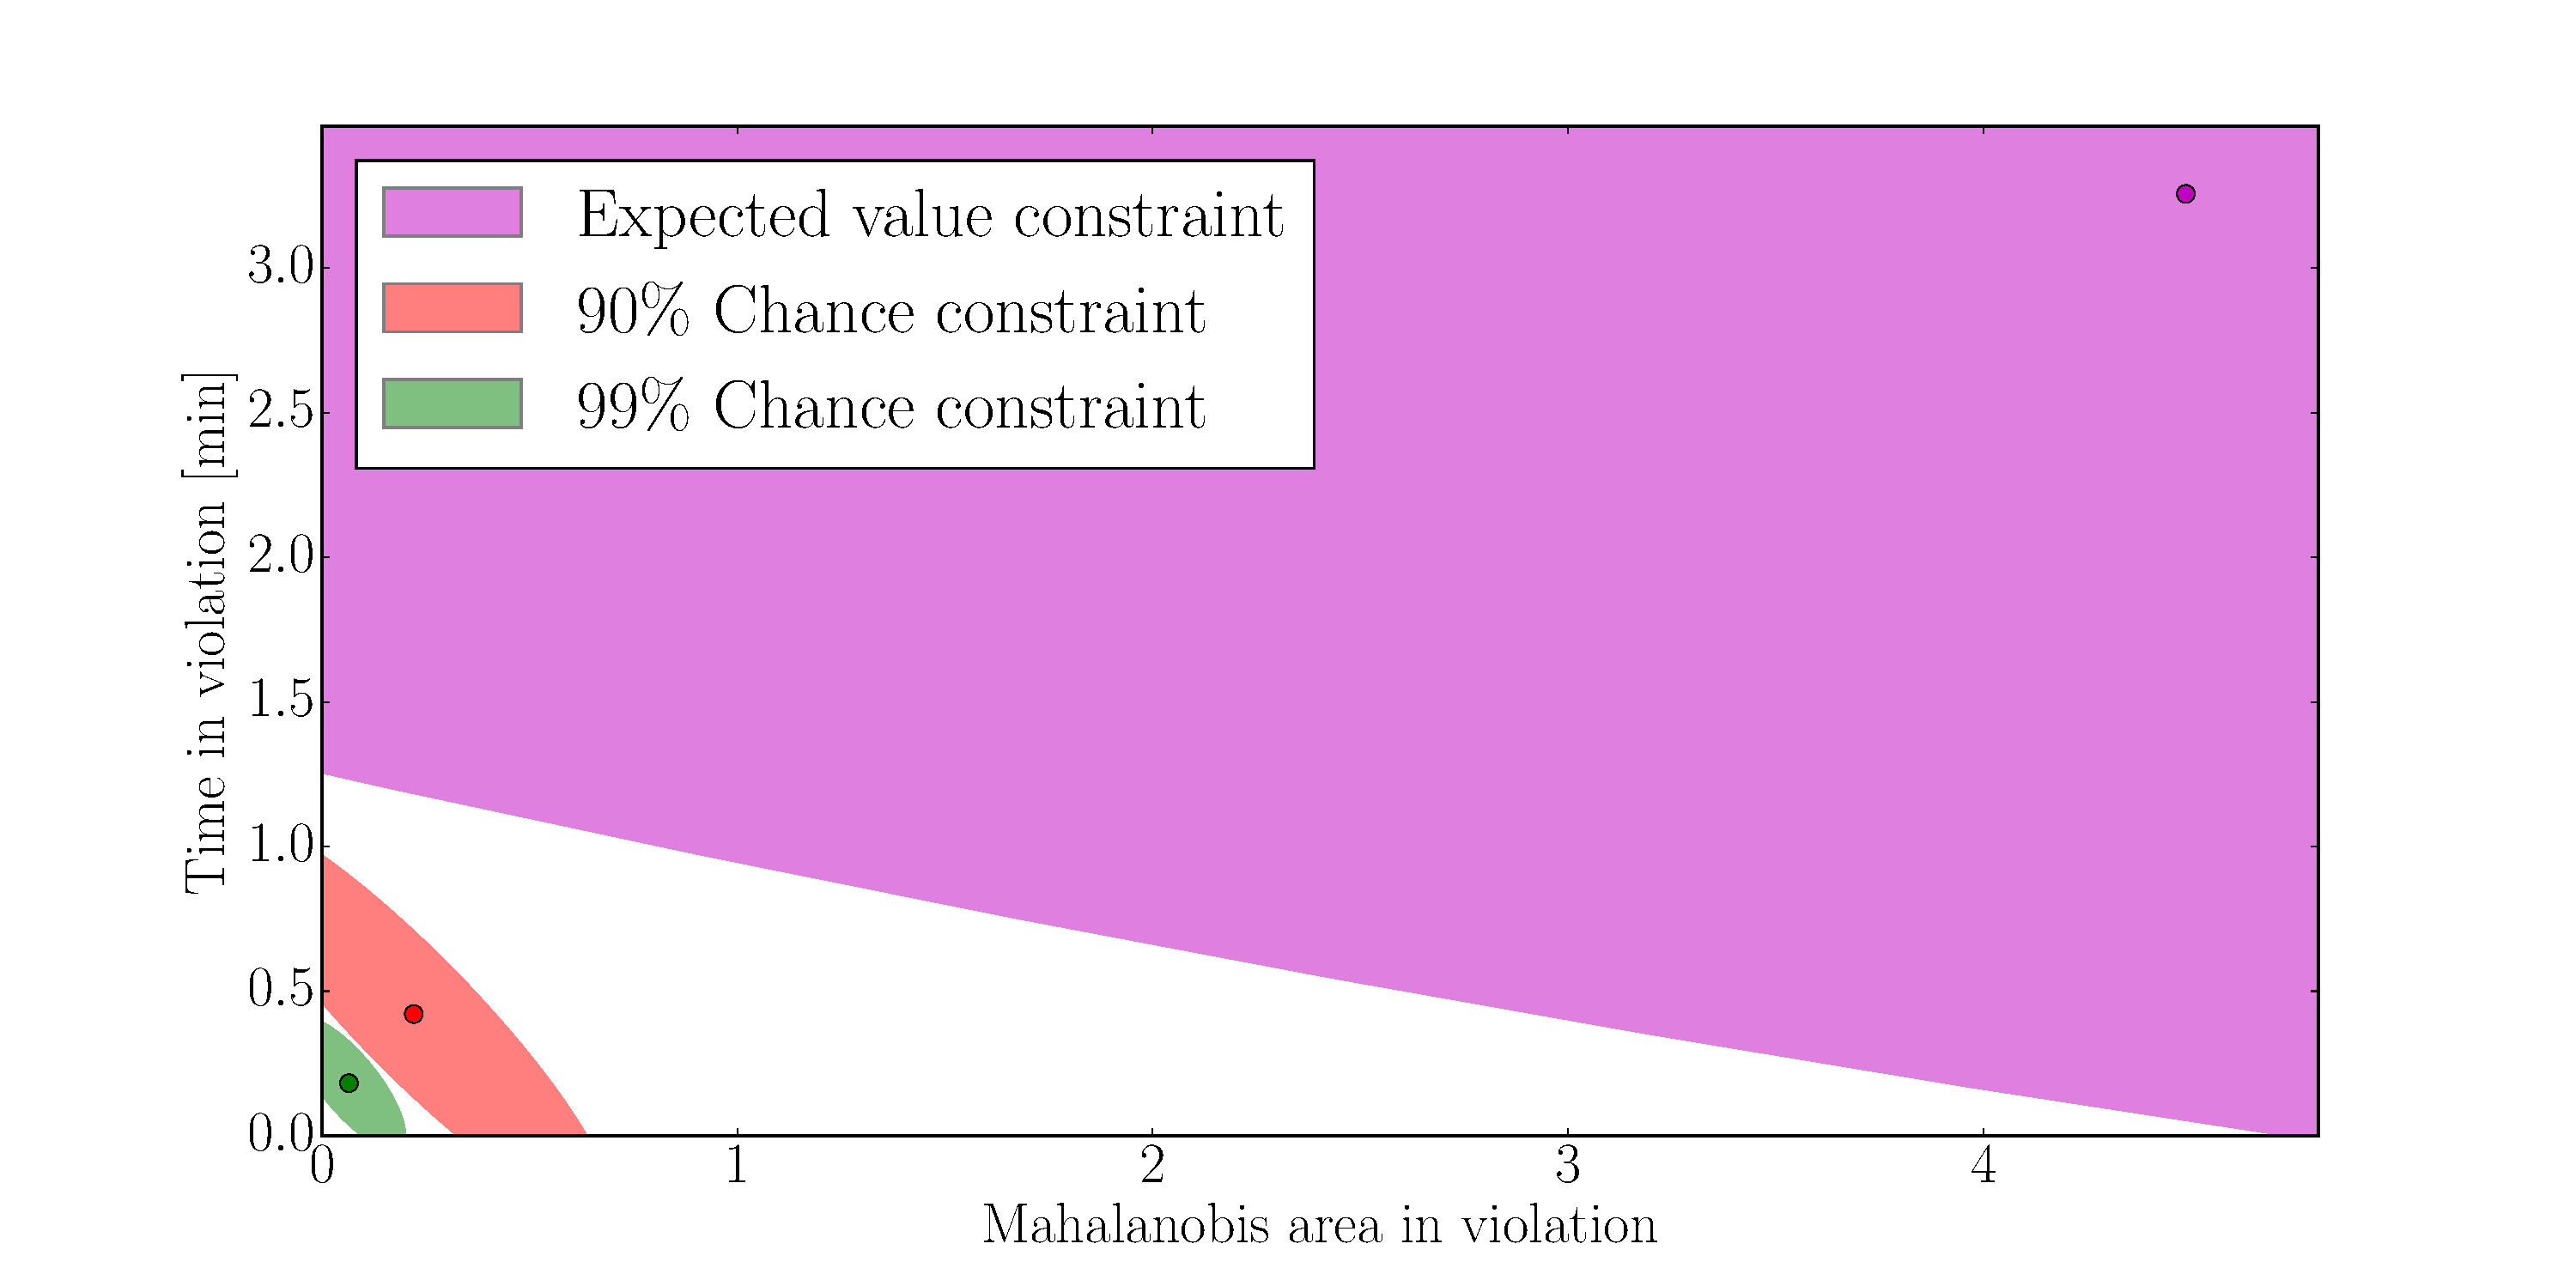
\includegraphics[width=\textwidth]{spf_mc.pdf}
\caption{Monte Carlo analysis of the switching controller algorithm applied within the context of the expected value and chance constrained MPCs developed in chapter \ref{sec_linear_control}. Each shaded region is where 90\% of the simulations scored.}
\label{fig_spf_mc}
\end{figure}
Like in chapter \ref{sec_linear_control} we see a clear benefit in increasing the chance constraint threshold: the higher the threshold the less the constraint is violated both in time and in severity. Figure~\ref{fig_spf_mc2} illustrates that we also have set point tracking. A Monte Carlo simulation using 50 runs each is plotted for each switching controller to illustrate their effectiveness.
\begin{figure}[H] 
\centering
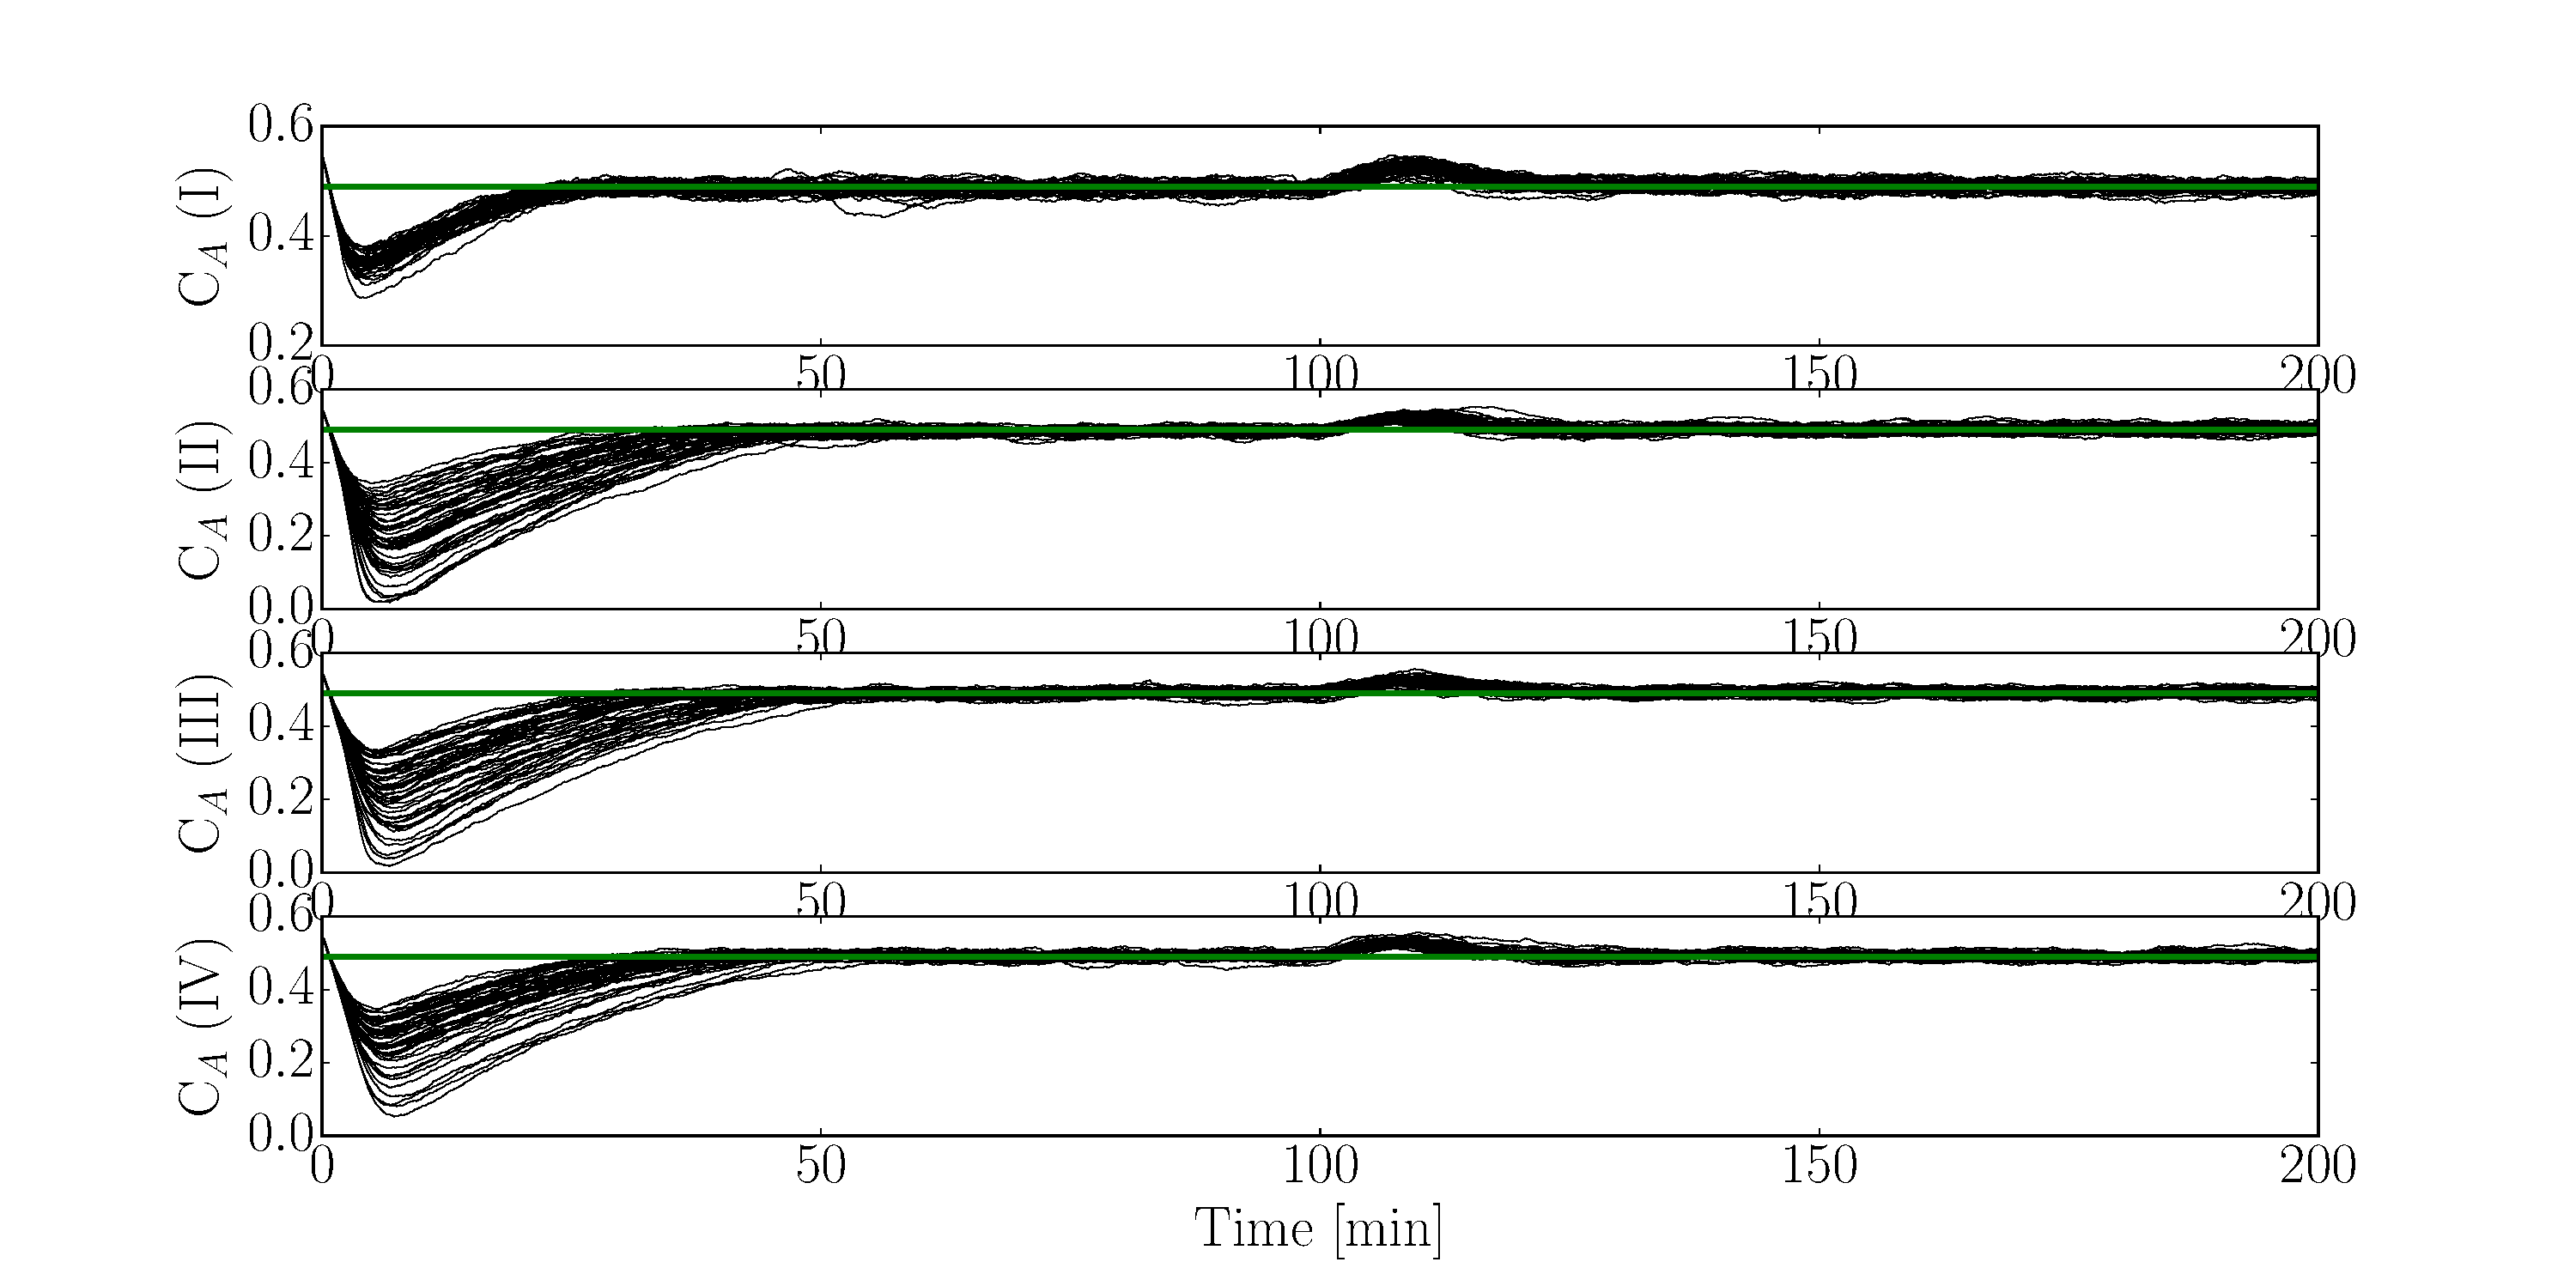
\includegraphics[width=\textwidth]{spf_mc2.pdf}
\caption{Monte Carlo set point tracking for the switching controllers. Subplot (I) shows the set point tracking of the switching LQG controller. Suplots (II), (III) and (IV) show the set point tracking of the expected value, 90\% chance and 99\% chance constrained switching MPC controllers. The green line is the set point.}
\label{fig_spf_mc2}
\end{figure}
In figure \ref{fig_spf_mc2} we clearly see a concentration tracking bump after about 100 minutes - when the controller breaks. After that it is clear that the controller has switched because we again have set point tracking. The Monte Carlo absolute set point error over the last 10 minutes of each simulation is 1.30\%, 1.64\%, 1.47\% and 1.42\% for the LQG controller, the expected value-, 90\% chance- and 99\% chance constrained MPC controllers. 

It is interesting that the same trends observed in chapter \ref{sec_linear_control} are evident here. The chance constrained MPC controllers show better tracking error than the expected value controller. Again the aggressiveness of the expected value controller causes the higher error. In all cases we have set point tracking (a small $\delta$ as per definition \ref{def_stoch_ref_track_goal}) despite the plant fault.

\section{Conclusion}
In this chapter we have developed a switching controller algorithm which detects when a process fault has occurred by using noisy measurement data in conjunction with a switching particle filter. The controller uses this knowledge to adapt the model used for control. The switching particle filter successfully identified when the modelled fault occurred in all the simulations.

The LQG controller, expected value- and chance constrained MPC controllers were all implemented within the switching controller algorithm framework. It was found that they were able to stabilise and control the system to set point despite the plant fault. This is was confirmed using Monte Carlo analysis. Furthermore, the scheme is computationally efficient because the controllers can be formulated as deterministic, linearly constrained quadratic programming optimisation problems. 

The bottleneck in the switching controller algorithm is inference. Since it is essentially a particle filter it is reasonable to suppose that there might be problems in higher dimensional spaces. However, recent work \cite{daum} on particle filters looks extremely promising in reducing the computational problems associated with filters of this kind.